\setcounter{ex}{0}
\setcounter{dang}{0}
\Opensolutionfile{ans}[ans/CD3/Muc_9_10]
\section{Mức độ 9,10 điểm}
\begin{dang}{Xác định $m$ để GTLN-GTNN của hàm số chứa dấu giá trị tuyệt đối thỏa mãn điều kiện cho trước}
\end{dang}	
\begin{ex}%[2H1K3]
	[Đề Tham Khảo 2018-BGD]
	Gọi $S$ là tập hợp tất cả các giá trị của tham số thực $m$ sao cho giá trị lớn nhất của hàm số $y=\left|x^3-3x+m\right|$ trên đoạn $\left[0;2\right]$ bằng $3$. Số phần tử của $S$ là 
	\choice
	{ $1$}
	{\True $2$}
	{ $0$}
	{$6$}
	\loigiai{
		Xét hàm số $f(x) = x^3-3x + m$ với $x \in \left[0;2\right]$.\\
		Ta có $f'(x) = 3x^2 - 3$.\\
		$f'(x) = 0 \Leftrightarrow \hoac{&x = 1\\&x = -1 \notin \left[0;2\right]}$.\\
		Bảng biến thiên
		\begin{center}
			\begin{tikzpicture}
				\tkzTabInit[lgt=1.2,espcl=4]
				{$x$/1,$f’(x)$/1,$f(x)$/2}
				{$0$,$1$,$2$}
				\tkzTabLine{ ,-,z,+, }
				\tkzTabVar{+/$m$,-/$m - 2$,+/$m + 2$}
			\end{tikzpicture}
		\end{center}
		Vậy $ m - 2 \le f(x) \le m + 2$ với mọi $x$ thuộc đoạn $\left[0;2\right]$.\\
		Suy ra $ \displaystyle \max _{\left[0;2 \right]  }{ y }= \max{\left \{ \left|m -2 \right|; \left|m+2\right| \right\}}$.
		\begin{itemize}
			\item Trường hợp 1: $m \ge 0$ khi đó $ \displaystyle \max _{\left[0;2 \right]  }{ y }=m+2=3 \Leftrightarrow m=1$.
			\item Trường hợp 2: $m<0$ khi đó $ \displaystyle \max _{\left[0;2 \right]  }{ y }=2-m=3 \Leftrightarrow m=-1$.
		\end{itemize}
	}
\end{ex}
\begin{ex}%[Đề minh họa 2020]%[2D1G3-1]
	Gọi $S$ là tập hợp tất cả các giá trị thực của tham số $m$ sao cho giá trị lớn nhất của hàm số $f(x)=\left| x^3-3x+m \right|$ trên đoạn $\left[ 0;3 \right]$ bằng $16$. Tổng tất cả các phần tử của $S$ bằng
	\choice
	{\True $-16$}
	{$16$}
	{$-12$}
	{$-2$}
	\loigiai{
		Xét hàm số $g(x)=x^3-3x+m$ trên $\left[ 0;3 \right]$.\\
		Ta có $g'(x) = 3x^2 - 3$.\\
		$g'(x) = 0 \Leftrightarrow \hoac{&x = 1\\&x = -1 \notin \left[0; 3\right].}$\\
		Bảng biến thiên
		\begin{center}
			\begin{tikzpicture}
				\tkzTabInit[lgt=1.2,espcl=4]
				{$x$/1,$g’(x)$/1,$g(x)$/2}
				{$0$,$1$,$3$}
				\tkzTabLine{ ,-,z,+, }
				\tkzTabVar{+/$m$,-/$m - 2$,+/$m + 18$}
			\end{tikzpicture}
		\end{center}
		Vậy $ m - 2 \le g(x) \le m + 18$ với mọi $x$ thuộc đoạn $\left[0; 3\right]$.\\
		Suy ra $\heva{&\displaystyle \max _{\left[0; 3 \right]  }{g(x)}= \max\{g(0), g(1), g(3) \} = \max \{m, m - 2, m + 18\} = m + 18\\&\displaystyle \min _{\left[0; 3 \right]  }{g(x)}= \min{\left \{ g(0), g(1), g(3) \right\}} =  \min \{m, m - 2, m + 18\} = m - 2.} $\\
		Suy ra $\max _{\left[0; 3 \right]  }{f(x)} = \max \{|m -2|, |m + 18|\} = 16 \Leftrightarrow \hoac{&\heva{& |m + 18| = 16\\&|m + 18| \geq |m - 2|}\\&\heva{& |m - 2| = 16\\&|m - 2| \geq |m + 18|}} \Leftrightarrow \hoac{&m = -2\\&m = -14.}$\\
		Vậy tổng các phần tử của $S$ bằng $-14 + \left( -2 \right) = -16 $.
	}
\end{ex}
\begin{ex}%[Nguyễn Thế Út]%[2D1G3-1]
	Cho hàm số $ y=\dfrac{x+m}{x+1} $ ($ m $ là tham số thực). Gọi $ S $ là tập hợp tất cả các giá trị của $m$ sao cho $\max\limits_{[0;1]}|f(x)|+\min\limits_{[0;1]}|f(x)|=2$. Số phần tử của $ S $ là 
	\choice
	{$ 6 $}
	{\True $ 2 $}
	{$ 1 $}
	{$ 4 $}
	\loigiai{
		Ta có $f'(x) = \dfrac{1-m}{(x+1)^2}$.
		\begin{itemize}
			\item Nếu $ m=1 $ thì $f(x)=\dfrac{x+1}{x+1}=1,\forall x\neq -1$. Khi đó $\max\limits_{[0;1]}|f(x)|+\min\limits_{[0;1]}|f(x)|=2$ (thỏa mãn).\\
			Do đó $ m=1 $ thỏa mãn bài toán.
			\item Nếu $ m\neq 1 $ thì hàm số đơn điệu trên $ [0;1] $.
			\begin{enumerate}[TH 1.]
				\item $\left(\dfrac{m+1}{2}\right)\cdot m \le 0$ thì $\min\limits_{[0;1]}|f(x)| = 0,\max\limits_{[0;1]}|f(x)|=\max\left\{\dfrac{|m+1|}{2};|m|\right\}$.\\
				Do đó 
				\begin{align*}
					\max\limits_{[0;1]}|f(x)|+\min\limits_{[0;1]}|f(x)|=2&\Leftrightarrow 0+\dfrac{\left|\dfrac{m+1}{2}+m\right|+\left|\dfrac{m+1}{2}-m\right|}{2}=2\\
					&\Leftrightarrow\dfrac{|3m+1|+|m-1|}{4}=2\Leftrightarrow\left[\begin{array}{l}
						m\ge 1:m=2 (\text{ loại})  \\
						1>m\geq -\dfrac{1}{3}:m=3(\text{ loại})\\
						m<-\dfrac{1}{3}:m=-2(\text{ loại})
					\end{array}\right.
				\end{align*}
				\item $\left(\dfrac{m+1}{2}\right)\cdot m> 0$ thì $\min\limits_{[0;1]}|f(x)|=\min\left\{\dfrac{|m+1|}{2};|m|\right\},\max\limits_{[0;1]}|f(x)|=\max\left\{\dfrac{|m+1|}{2};|m|\right\}$.\\
				Do đó 
				\begin{align*}
					&\max\limits_{[0;1]}|f(x)|+\min\limits_{[0;1]}|f(x)|=2\\
					&\Leftrightarrow\dfrac{\left|\left|\dfrac{m+1}{2}+m\right|-\left|\dfrac{m+1}{2}-m\right|\right|}{2}+\dfrac{\left|\dfrac{m+1}{2}+m\right|+\left|\dfrac{m+1}{2}-m\right|}{2}=2\\
					&\Leftrightarrow\dfrac{\left||3m+1|-|m-1|\right|}{4}+\dfrac{|3m+1|+|m-1|}{4}=2\\
					&\Leftrightarrow\hoac{&|3m+1|\geq |m+1|:2|3m+1|=8&(2)\\&|3m+1|<|m+1|:2|m-1|=8&(3)}
				\end{align*}
				Giải $(2)\Leftrightarrow\left[\begin{array}{l}
					m=1 (\text{ thỏa})\\
					m=-\dfrac{5}{3}(\text{thỏa mãn}).
				\end{array}\right.$\\
				Giải $(3)\Leftrightarrow\left[\begin{array}{l}
					m=5(\text{ loại})\\
					m=-3(\text{ loại}).
				\end{array}\right.$
			\end{enumerate} 
			Vậy $S=\left\{1;\dfrac{-5}{3}\right\}$. Suy ra số phần tử của $S$ là $2$.
		\end{itemize}
	}	
\end{ex}
\begin{ex}%[2D1G3-1] % Câu 4.
	Tìm $m$ để giá trị lớn nhất của hàm số $y = |x^3 - 3x + 2m - 1|$ trên đoạn $[0; 2 ]$ là nhỏ nhất. Giá trị của $m$ thuộc khoảng nào?
	\choice
	{ $\left(-\dfrac{3}{2}; -1 \right)$}
	{ $\left(\dfrac{2}{3}; 2 \right)$}
	{ $[-1; 0 ]$}
	{\True $(0; 1)$}
	\loigiai{
		Xét hàm số $y = f(x) = x^3 - 3x + 2m - 1$ trên đoạn $[0; 2]$.\\
		Ta có $ f'(x) = 3x^2 - 3 = 0 \Leftrightarrow \hoac{& x = -1 \notin [0; 2] \\ & x = 1.}$\\
		Ta có $f(0) = 2m - 1$, $f(1) = 2m - 3$ và $f(2) = 2m + 1$.\\
		Suy ra $\max\limits_{[0;3]}|f(x)|  = \max\{ |2m - 1|; |2m - 3|; |2m + 1| \} = \max \{ | 2m - 3 |;| 2m + 1 | \} = P$.
		\begin{itemize}
			\item \textbf{Trường hợp 1:} Nếu $| 2m - 3 |\ge | 2m + 1 |\Leftrightarrow -4(4m - 2) \ge 0\Leftrightarrow m \le \dfrac{1}{2}$.\\
			Khi đó $P = | 2m - 3 |\ge 2$,$\forall m \le \dfrac{1}{2}$. Suy ra ${\mathrm{P}_{\min }} = 2 \Leftrightarrow m = \dfrac{1}{2}$.
			\item \textbf{Trường hợp 2:} Nếu $| 2m-3 |<| 2m + 1 | \Leftrightarrow -4( 4m-2 )<0\Leftrightarrow m > \dfrac{1}{2}$.\\
			Khi đó $P=| 2m+1 |>2$, $\forall m > \dfrac{1}{2}$. Suy ra ${\mathrm{P}_{\min }}$ không tồn tại.
		\end{itemize}
		Vậy $m = \dfrac{1}{2}$.
	}
\end{ex}
\begin{ex}%[2D1G3-1] % Câu 5.
	Tính tổng tất cả các giá trị của tham số $m$ sao cho giá trị lớn nhất của hàm số $y = |x^2 - 2x + m|$ trên đoạn $[-1; 2]$ bằng $5$.
	\choice
	{ $-1$}
	{ $2$}
	{\True $-2$}
	{ $1$}
	\loigiai{
		Ta có $y' = \dfrac{2x - 2}{| x^2 - 2x + m |}$.\\
		Khi đó $y' = 0 \Rightarrow x = 1$.\\
		Yêu cầu bài toán $ \Leftrightarrow \max \{ y(-1), y(2), y(1) \} = 5 \Leftrightarrow \max \{ | 3 + m |, | m |, | m - 1 | \} = 5$.
		\begin{itemize}
			\item \textbf{Trường hợp 1:} Nếu $ m \ge -1$, ta có $\max \{ | 3+m |,| m |,| m-1 | \}=5\Leftrightarrow | 3 + m |= 5 \Rightarrow m=2$.
			\item \textbf{Trường hợp 2:} Nếu $ m < -1$, ta có $\max \{ | 3 + m |,| m |,| m - 1 | \}=5\Leftrightarrow | m - 1 |= 5 \Rightarrow m = -4$
		\end{itemize}
		Vậy tổng các giá trị $ m$ bằng $-2$.
	}
\end{ex}
\begin{ex}%[2D1G3-1] % Câu 6.
	Cho hàm số $y = |x^2 + 2x + a - 4|$ ($a$ là tham số ). Tìm $a$ để giá trị lớn nhất của hàm số trên đoạn $[-2; 1]$ đạt giá trị nhỏ nhất.
	\choice
	{ $a = 1$}
	{\True $a = 3$}
	{ $a = 2$}
	{ $a = 5$}
	\loigiai{
		Hàm số đã cho xác định và liên tục trên $[-2; 1]$.\\
		Ta có $y = |x^2 + 2x + a - 4| = | (x + 1)^2 + a - 5 | \;\; (*)$.\\
		Đặt $t = (x + 1)^2$. Do $x \in [-2; 1] \Rightarrow t \in [0; 4]$.\\
		Lúc đó hàm số đã cho trở thành $ f(t) = | t + a - 5 |$ với $ t \in [0; 4]$.\\
		Suy ra
		\allowdisplaybreaks
		\begin{eqnarray*}
			\max\limits_{x \in [-2; 1]} y = \max\limits_{t \in [0; 4]} f(t) 
			&=& \max\limits_{t \in [0; 4]} f(t) \{ f(0); f(4) \}\\
			&=& \max\limits_{t \in [0; 4]} \{ | a - 5 |; | a - 1 | \}\\
			&\ge& \dfrac{| a - 1 | + | a - 5 |}{2}\\
			&\ge& \dfrac{| a - 1 + 5 - a |}{2} = 2.
		\end{eqnarray*}
		Đẳng thức xảy ra khi $| a-1 |=| a-5 |=2\Leftrightarrow a=3$.\\
		Do đó giá trị nhỏ nhất của $\underset{t\in [ 0;4 ]}{\mathop{\max f( t )}}$ là $2$ khi $ a=3$.
	}
\end{ex}
\begin{ex}%[2D1G3-1] % Câu 7.
	Gọi $S$ là tập hợp tất cả các giá trị thực của tham số $ m$ sao cho giá trị lớn nhất của hàm số $y = \left| \dfrac{x^2 + mx + m}{x + 1} \right|$ trên $[1; 2]$ bằng $2$. Số phần tử của tập $S$ là
	\choice
	{ $3$}
	{ $1$}
	{ $4$}
	{\True $2$}
	\loigiai{
		Xét hàm số $y = \dfrac{x^2 + mx + m}{x + 1}$ trên $[1; 2]$.\\
		Ta có $f'(x) = \dfrac{x^2 + 2x}{(x + 1)^2}$.\\
		Khi $f'(x) = 0 \Leftrightarrow \hoac{& x = 0 \notin [1; 2] \\ & x = -2 \notin [1; 2]}$.\\
		Mà $ f(1) = \dfrac{2m + 1}{2}$, $f(2) = \dfrac{3m + 4}{3} \Rightarrow \max\limits_{x \in [1; 2]} y = \left\{ \left| \dfrac{2m+1}{2} \right|; \left| \dfrac{3m + 4}{3} \right| \right\}$.\\
		\textbf{Trường hợp 1:} $\max\limits_{x \in [1; 2]} y = \left| \dfrac{2m+1}{2} \right| = 2 \Rightarrow \hoac{& m = \dfrac{3}{2} \\ & m = -\dfrac{5}{2}.}$\\
		• Với $m = \dfrac{3}{2} \Rightarrow \left| \dfrac{3m+4}{3} \right| = \dfrac{17}{6}>2$ (loại).\\
		• Với $ m = -\dfrac{5}{2} \Rightarrow \left| \dfrac{3m+4}{3} \right| = \dfrac{7}{6}<2$ (thỏa mãn).\\
		\textbf{Trường hợp 2:} $\max\limits_{x \in [1; 2]} y = \left| \dfrac{3m + 4}{3} \right| = 2 \Rightarrow \hoac{& 3m + 4 = 6 \\ & 3m + 4 =-6 }\Leftrightarrow \hoac{& m = \dfrac{2}{3} \\ & m = -\dfrac{10}{3}. }$\\
		• Với $ m= \dfrac{2}{3} \Rightarrow \left| \dfrac{2m+1}{2} \right| = \dfrac{7}{6}<2$ (thỏa mãn).\\
		• Với $ m= -\dfrac{10}{3} \Rightarrow \left| \dfrac{2m + 1}{2} \right| = \dfrac{17}{6}>2$ (loại).\\
		Vậy có $2$ giá trị của $m$ thỏa mãn.
	}
\end{ex}
\begin{ex}%[2D1G3-1] % Câu 8.
	Xét hàm số $ f(x) = |x^2 + ax + b |$, với $a$, $b$ là tham số. Gọi $M$ là giá trị lớn nhất của hàm số trên $[-1; 3]$. Khi $M$ nhận giá trị nhỏ nhất có thể được, tính $a + 2b$.
	\choice
	{ $2$}
	{ $4$}
	{\True $-4$}
	{ $3$}
	\loigiai{
		Xét hàm số $ f(x) = |x^2 + ax + b|$.\\
		Theo đề bài, $M$ là giá trị lớn nhất của hàm số trên $[-1; 3]$.\\
		Suy ra 
		\allowdisplaybreaks
		\begin{eqnarray*}
			\heva{& M \ge f(-1) \\ & M \ge f(3) \\ & M \ge f(1)} 
			&\Leftrightarrow& \heva{& M \ge | 1-a+b | \\ & M \ge | 9+3a+b | \\ & M \ge | 1+a+b |}\\
			&\Rightarrow& 4M \ge | 1-a+b |+| 9+3a+b |+2| -1-a-b |\\
			&\geq& | 1-a+b+9+3a+b+2(-1-a-b) |\\
			&\Rightarrow& 4M \ge 8\\
			&\Rightarrow& M \ge 2.
		\end{eqnarray*}
		Nếu $M = 2$ thì điều kiện cần là $| 1-a+b |=| 9+3a+b |=| -1-a-b |=2$ và $1-a+b$, $9+3a+b$, $-1-a-b$ cùng dấu $\Leftrightarrow 
		\hoac{&1-a+b=9+3a+b=-1-a-b=2 \\ & 1-a+b=9+3a+b=-1-a-b=-2}
		\Leftrightarrow \heva{& a = -2 \\ & b = -1.}$\\
		Ngược lại khi $\heva{&a = -2 \\ & b = -1 }$ ta có, hàm số $ f(x) = |x^2 -2x-1 |$ trên $[-1; 3]$.\\
		Xét hàm số $ g(x) = x^2 - 2x - 1$ xác định và liên tục trên $[-1; 3]$.\\
		Ta có $g'(x) = 2x - 2$.\\
		$g'(x) = 0 \Leftrightarrow x = 1 \in [-1; 3]$.\\
		Do $M = \max\limits_{x \in [-1; 3]} f(x) \Rightarrow M = \max \{ | g(-1)|; |g(3)|; |g(1)| \} = 2$.\\
		Vậy $\heva{& a=-2 \\ & b=-1.}$\\
		Ta có: $ a + 2b = -4$.
	}
\end{ex}
\begin{ex}%[2D1G3-1] % Câu 9.
	Cho hàm số $ y = | x^3 + x^2 + m^2 + 1)x + 27|$. Giá trị lớn nhất của hàm số trên đoạn $[-3; -1]$ có giá trị nhỏ nhất bằng
	\choice
	{ $26$}
	{\True $18$}
	{ $28$}
	{ $16$}
	\loigiai{
		Xét hàm số $ u = x^3 + x^2 + (m^2 + 1)x + 27$ trên đoạn $[-3; -1]$.\\
		Ta có $u'= 3x^2 + 2x + m^2 + 1 > 0, \forall x \in [-3; -1]$.\\
		Do đó $A = \max\limits_{x \in [-3; -1]} u = u(-1) = 26 - m^2$; $ a = \min\limits_{x \in [-3; -1]} u = u(-3) = 6 - 3m^2$.\\
		Do $M = \max\limits_{x \in [-3; -1]} y = \max \{ | 26 - m^2 |,| 6 - 3m^2 | \}$ và $4M \ge 3| 26 - m^2 | + | 6 - 3m^2 | \ge 72$.\\
		Vậy $M \ge 18$.\\
		Dấu bằng xảy ra khi $| 26 - m^2 | = | 6 - 3m^2 | = 18 \Leftrightarrow m = \pm 2\sqrt {2}$.
	}
\end{ex}
\begin{ex}%[2D1G3-1] % Câu 10.
	Có bao nhiêu giá trị thực của tham số $m$ để giá trị lớn nhất của hàm số $ y = |x^2 + 2x + m - 4 |$ trên đoạn $[-2; 1]$ bằng $4$?
	\choice
	{ $1$}
	{\True $2$}
	{ $3$}
	{ $4$}
	\loigiai{
		Xét hàm số $f(x) = x^2 + 2x + m - 4$.\\
		Ta có $f'(x) = 2x + 2$.\\
		Do đó $f'(x) = 0 \Leftrightarrow x = -1$.\\
		Do đó $\max\limits_{x \in [-2; 1]} | x^2 + 2x + m - 4 | = \max \{ | m-1 |;| m-4 |;| m-5 | \}$.\\
		Ta thấy $m - 5 < m - 4 < m - 1$ với mọi $ m \in \mathbb{R}$.\\
		Suy ra $\max\limits_{x \in [-2; 1]} y$ chỉ có thể là $| m - 5 |$ hoặc $|m - 1 |$.\\
		Nếu $\max\limits_{x \in [-2; 1]} y = | m-5 |$ thì $\heva{& | m-5 |=4 \\ & | m-5 |\ge | m-1 | } \Leftrightarrow m = 1$.\\
		Nếu $\max\limits_{x \in [-2; 1]} y = | m - 1 |$ thì $\heva{& | m - 1 | = 4 \\ & | m - 1 |\ge | m - 5 | } \Leftrightarrow m = 5$.\\
		Vậy $ m \in \{ 1;5 \}$.
	}
\end{ex}

%%==========Câu 11
\begin{ex}%[2D1G3-1][Chuyên Nguyễn Thị Minh Khai - Sóc Trăng - 2018] 
	Gọi $S$ là tập hợp tất cả các giá trị của tham số $m$ sao cho giá trị lớn nhất của hàm số $y=\left| x^3-3x^2-9x+m \right|$ trên đoạn $[-2;4]$ bằng $16$. Số phần tử của $S$ là
	\choice
	{$0$}
	{$2$}
	{$4$}
	{\True $1$}
	\loigiai{
		Xét hàm số $f(x)=x^3-3x^2-9x+m$ trên đoạn $\left[-2;4\right]$.\\
		$f'=3x^2-6x-9$; $f'(x)=0\Leftrightarrow \left[ \begin{aligned}
			& x=-1 \\
			& x=3 \\
		\end{aligned} \right.$ (thỏa mãn).\\
		$f(-2)=-2+m$; $f(-1)=5+m$; $f(3)=-27+m$; $f(4)=-20+m$.\\
		$\Rightarrow \min\limits_{[-2;4]}f(x)=m-27$; $\max\limits_{[-2;4 ]}f(x)=m+5\Rightarrow \max\limits_{\left[-2;4 \right]}\left| f(x) \right|=\max \left\{ \left| m-27 \right|;\left| m+5 \right| \right\}$.\\
		\textbf{TH1:} Nếu $\left| m-27 \right|\le \left| m+5 \right| \;(*)$\\
		$\Rightarrow \max\limits_{[-2;4]}\left| f(x) \right|=\left| m+5 \right|\Rightarrow \left| m+5 \right|=16\Leftrightarrow \left[ \begin{aligned}
			& m=11 \\
			& m=-21 \\
		\end{aligned} \right.$. Đối chiếu điều kiện $(*)\Rightarrow m=11$.\\
		\textbf{TH2:} Nếu $\left| m-27 \right|>\left| m+5 \right|\; (**)$\\
		$\Rightarrow \max\limits_{[-2;4]}\left| f(x) \right|=\left| m-27 \right|\Rightarrow \left| m-27 \right|=16\Leftrightarrow \left[ \begin{aligned}
			& m=43 \\
			& m=11 \\
		\end{aligned} \right.$. (Không thỏa mãn điều kiện $\left( ** \right)$).\\
		Vậy $S=\left\{ 11 \right\}\Rightarrow S$ có $1$ phần tử.}
	
\end{ex}

%%==========Câu 12
\begin{ex}%[2D1G3-1][Chuyên Hạ Long 2018] 
	Gọi $S$ là tập tất cả các giá trị nguyên của tham số $m$ sao cho giá trị lớn nhất của hàm số $y=\left| \dfrac{1}{4}{x^4}-\dfrac{19}{2}{x^2}+30x+m-20 \right|$ trên đoạn $\left[0;2\right]$ không vượt quá $20$. Tổng các phần tử của $S$ bằng
	\choice
	{$210$}
	{$-195$}
	{\True $105$}
	{$300$}
	\loigiai{
		Xét hàm số $g(x)=\dfrac{1}{4}{x^4}-\dfrac{19}{2}{x^2}+30x+m-20$ trên đoạn $[0;2]$.\\
		Ta có $g'(x)=x^3-19x+30$; $g'(x)=0\Leftrightarrow \left[ \begin{aligned}
			& x=-5\notin [0;2] \\
			& x=2 \\
			& x=3\notin [0;2]. \\
		\end{aligned} \right.$\\
		Bảng biến thiên
		\begin{center}
			\begin{tikzpicture}
				\tkzTabInit[nocadre=false,lgt=1.2,espcl=2,deltacl=0.6]
				{$x$/.6,$g'(x)$/.6,$g(x)$/1.7}
				{$-\infty$,$-5$,$0$,$2$,$3$,$+\infty$}
				\tkzTabLine{,-,0,,,+,0,-,0,+}
				\fill[pattern  = north west lines] (T13) rectangle (N31);
				\fill[pattern  = north east lines] (N43) rectangle (T21);
				\draw[] (N31) to (N33) (N41) to (N43);
				\node[fill=white,above] (n1) at (N33) {$g(0)$};
				\node[fill=white,below](n2) at (N42) {$g(2)$};
				\draw[arrow style] (n1) to (n2);
			\end{tikzpicture}
		\end{center}
		$g(0)=m-20$; $g(2)=m+6$.\\
		Để $\max\limits_{\left[0;2\right]}\left| g(x) \right|\le 20$ thì $\left\{ \begin{aligned}
			& g(0)\le 20 \\
			& g(2)\le 20 \\
		\end{aligned} \right.$ $\Leftrightarrow \left\{\begin{aligned}
			& \left| m-20 \right|\le 20 \\
			& \left| m+6 \right|\le 20 \\
		\end{aligned} \right.\Leftrightarrow 0\le m\le 14$.\\
		Mà $m\in \mathbb{Z}$ nên $m\in \left\{ 0;1;2;...;14 \right\}$.\\
		Vậy tổng các phần tử của $S$ là $105$.}
\end{ex}

%%==========Câu 13
\begin{ex}%[2D1G3-1]
	Gọi $S$ là tập hợp tất cả các giá trị thực của tham số $m$ sao cho giá trị lớn nhất của hàm số
	$y=\left| \sin ^{2}x-2\sin x+m \right|$ bằng $1$. Số phần tử của $S$ là
	\choice
	{\True $0$}
	{$1$}
	{$4$}
	{$3$}
	\loigiai{
		Đặt $\sin x=t\,\left( t\in [-1;1] \right)\Rightarrow y=\left| {t^2}-2t+m \right|$.\\
		Xét hàm số $f(t)=t^2-2t+m$\\
		Có $f'(t)=2t-2=0\Leftrightarrow t=1 \in \left[-1;1\right]$;	$f(-1)=m+3,\,f(1)=m-1$.\\ 
		Khi đó $\left\{ \begin{aligned}
			& \max\limits_{[-1;1]} f(x)=\max \left\{ m+3;m-1 \right\}=m+3 \\
			& \min\limits_{[-1;1]}f(x)=\min \left\{ m+3;m-1 \right\}=m-1. \\
		\end{aligned} \right.$\\
		\textbf{TH1:} $\left| m+3 \right|\ge \left| m-1 \right|\Leftrightarrow m\ge -1$
		$\Rightarrow \max f(x)=\left| m+3 \right|=1\Leftrightarrow \left[ \begin{aligned}
			& m=-2 \text{ (loại)} \\
			& m=-4 \text{ (loại)}. \\
		\end{aligned} \right.$\\
		\textbf{TH1}: $\left| m+3 \right|<\left| m-1 \right|\Leftrightarrow m<-1$
		$\Rightarrow \max f(x)=\left| m-1 \right|=1\Leftrightarrow \left[ \begin{aligned}
			& m=2 \text{ (loại)} \\
			& m=0 \text{ (loại)}. \\
		\end{aligned} \right.$\\
		Suy ra không tồn tại $m$ thỏa mãn.}
\end{ex}

%%==========Câu 14
\begin{ex}%[2D1G3-1][Chuyên Hưng Yên - 2020] 
	Cho hàm số $y=\left| \dfrac{x^4+ax+a}{x+1} \right|$, với $a$ là tham số thực. Gọi $M$, $m$ lần lượt là giá trị lớn nhất và giá trị nhỏ nhất của hàm số đã cho trên đoạn $\left[1;2\right]$. Có bao nhiêu giá trị nguyên của tham số $a$ để $M\ge 2m$?
	\choice
	{$10$}
	{\True $14$}
	{$5$}
	{$20$}
	\loigiai{
		Xét hàm số $y=\dfrac{x^4+ax+a}{x+1}=\dfrac{x^4}{x+1}+a$.\\
		Ta có $y'=\dfrac{3x^4+4x^3}{{{\left( x+1 \right)}^2}}\Rightarrow y'=0\Leftrightarrow \left[ \begin{aligned}
			& x=-\dfrac{4}{3} \\
			& x=0. \\
		\end{aligned} \right.$\\
		Bảng biến thiên
		\begin{center}
			\begin{tikzpicture}[node style/.style={fill opacity=0,text opacity=1}] 
				%\tkzTabColors[backgroundcolor=yellow]
				\tkzTabInit[nocadre=false,lgt=1.2,espcl=2.25,deltacl=0.6]
				{$x$/.7,$y'$/.7,$y$/1.5}{$-\infty$,$-\frac{4}{3}$,$-1$,$0$,$+\infty$}
				\tkzTabLine{,+,z,-,d,-,z,+,} 
				\tkzTabVar{-/$-\infty$,+/$ $,-D+/$-\infty$/$+\infty$,-/$ $,+/$+\infty$}
			\end{tikzpicture}
		\end{center}
		Dựa vào bảng biến thiên suy ra $M=\max \left\{ \left| a+\dfrac{1}{2} \right|;\left| a+\dfrac{16}{3} \right| \right\}$ và $m=\min \left\{ \left| a+\dfrac{1}{2} \right|;\left| a+\dfrac{16}{3} \right| \right\}$.\\
		\textbf{TH1:} $a+\dfrac{1}{2}\ge 0\Leftrightarrow a\ge -\dfrac{1}{2}\Rightarrow \left\{ \begin{aligned}
			& M=\left| a+\dfrac{16}{3} \right|=a+\dfrac{16}{3} \\
			& m=\left| a+\dfrac{1}{2} \right|=a+\dfrac{1}{2}. \\
		\end{aligned} \right.$\\
		Khi đó $M\ge 2m\Leftrightarrow a+\dfrac{16}{3}\ge 2\left( a+\dfrac{1}{2} \right)\Leftrightarrow a\le \dfrac{13}{3}$.\\
		Kết hợp điều kiện, ta có $-\dfrac{1}{2}\le a\le \dfrac{13}{3}\Rightarrow $ có $5$ giá trị nguyên thỏa mãn điều kiện.\\
		\textbf{TH2:} $a+\dfrac{16}{3}\le 0\Leftrightarrow a\le -\dfrac{16}{3}\Rightarrow \left\{ \begin{aligned}
			& M=\left| a+\dfrac{1}{2} \right|=-a-\dfrac{1}{2} \\
			& m=\left| a+\dfrac{16}{3} \right|=-a-\dfrac{16}{3}. \\
		\end{aligned} \right.$\\
		$M\ge 2m\Leftrightarrow -a-\dfrac{1}{2}\ge 2\left( -a-\dfrac{16}{3} \right)\Leftrightarrow a\ge -\dfrac{61}{6}$.
		Kết hợp điều kiện ta có $-\dfrac{61}{6}\le a\le -\dfrac{16}{3}$. Suy ra có $5$ giá trị nguyên của $a$ thỏa mãn.\\
		\textbf{TH3:} $\left\{ \begin{aligned}
			& a+\dfrac{1}{2}<0 \\
			& a+\dfrac{16}{3}>0 \\
		\end{aligned} \right.\Leftrightarrow -\dfrac{16}{3}<a<-\dfrac{1}{2}$.\\
		Nếu $\left| a+\dfrac{1}{2} \right|>\left| a+\dfrac{16}{3} \right|\Leftrightarrow -a-\dfrac{1}{2}>a+\dfrac{16}{3}\Leftrightarrow a<-\dfrac{35}{12}$ thì
		$\left\{ \begin{aligned}
			& M=-a-\dfrac{1}{2} \\
			& m=a+\dfrac{16}{3} \\
		\end{aligned} \right.$\\
		$\Rightarrow M\ge 2m\Leftrightarrow -a-\dfrac{1}{2}\ge 2\left( a+\dfrac{16}{3} \right)\Leftrightarrow a\le -\dfrac{67}{18}$.\\
		Kết hợp điều kiện, ta có $-\dfrac{16}{3}<a\le -\dfrac{67}{18}$.	Suy ra có $2$ giá trị nguyên của $a$ thỏa mãn điều kiện.\\
		Nếu $\left| a+\dfrac{1}{2} \right|\le \left| a+\dfrac{16}{3} \right|\Leftrightarrow -a-\dfrac{1}{2}\le a+\dfrac{16}{3}\Leftrightarrow a\ge -\dfrac{35}{12}$ thì
		$\left\{ \begin{aligned}
			& M=a+\dfrac{16}{3} \\
			& m=-a-\dfrac{1}{2} \\
		\end{aligned} \right.$\\
		$\Rightarrow M\ge 2m\Leftrightarrow a+\dfrac{16}{3}\ge 2\left( -a-\dfrac{1}{2} \right)\Leftrightarrow a\ge -\dfrac{19}{9}$.
		Kết hợp điều kiện, ta có $-\dfrac{19}{9}\le a<-\dfrac{1}{2}$. Suy ra có $2$ giá trị nguyên của $a$ thỏa mãn điều kiện.\\
		Vậy có $14$ giá trị nguyên của $a$ thỏa mãn điều kiện.}
\end{ex}

%%==========Câu 15
\begin{ex}%[2D1G3-1][Chuyên Lương Văn Chánh - Phú Yên - 2020] 
	Gọi $S$ là tập hợp tất cả các giá trị nguyên của tham số thực $m$ sao cho giá trị lớn nhất của hàm số $y=\left| \dfrac{1}{4}{x^4}-14x^2+48x+m-30 \right|$ trên đoạn $\left[0;2\right]$ không vượt quá $30$. Tổng giá trị các phần tử của tập hợp $S$ bằng bao nhiêu?
	\choice
	{$120$}
	{$210$}
	{$108$}
	{\True $136$}
	\loigiai{
		Đặt $f(x)=\dfrac{1}{4}{x^4}-14x^2+48x+m-30$ là hàm số xác định và liên tục trên $[0;2]$.\\
		Với mọi $x\in [0;2]$ ta có $f'(x)=0\Leftrightarrow {x^3}-28x+48=0\Leftrightarrow x=2$.\\
		Suy ra $\max\limits_{[0;2]}\left| f(x) \right|=\max \left\{ \left| f(0) \right|;\left| f(2) \right| \right\}$.\\
		Theo đề $\max\limits_{[0;2]}\left| f(x) \right|\le 30\Leftrightarrow \left[ \begin{aligned}
			& \left\{ \begin{aligned}
				& \left| m-30 \right|\le 30 \\
				& \left| m+14 \right|\le \left| m-30 \right| \\
			\end{aligned} \right. \\
			& \left\{ \begin{aligned}
				& \left| m+14 \right|\le 30 \\
				& \left| m-30 \right|\le \left| m+14 \right| \\
			\end{aligned} \right. \\
		\end{aligned} \right.\Leftrightarrow \left\{ \begin{aligned}
			& \left| m-30 \right|\le 30 \\
			& \left| m+14 \right|\le 30 \\
		\end{aligned} \right.$\\
		$\Leftrightarrow \left\{ \begin{aligned}
			& -30\le m-30\le 30 \\
			& -30\le m+14\le 30 \\
		\end{aligned} \right.\Leftrightarrow \left\{ \begin{aligned}
			& 0\le m\le 60 \\
			& -44\le m\le 16 \\
		\end{aligned} \right.\Leftrightarrow 0\le m\le 16$.\\
		Do $m\in \mathbb{Z}\Rightarrow m\in S=\left\{ 0;1;2;...;16 \right\}$.\\
		Vậy tổng tất cả $17$ giá trị trong tập $S$ là $136$.}
\end{ex}

%%==========Câu 16
\begin{ex}%[2D1G3-1][Chuyên Lương Văn Tỵ - Ninh Bình - 2020] 
	Cho hàm số $f(x)=\left| 3{e^{4x}}-4{e^{3x}}-24{e^{2x}}+48e^x+m \right|$. Gọi $A$, $B$ lần lượt là giá trị lớn nhất và giá trị nhỏ nhất của hàm số đã cho trên $\left[0;\ln 2\right]$. Gọi $S$ là tập hợp tất cả các giá trị nguyên của tham số $m$ thuộc $\left[-23;10\right)$ thỏa mãn $A\le 3B$. Tổng các phần tử của tập $S$ bằng
	\choice
	{\True $-33$}
	{$0$}
	{$-111$}
	{$-74$}
	\loigiai{
		Đặt $t=e^x$, $x\in \left[ 0;\ln 2 \right]\Rightarrow t\in [1;2]$.\\
		Xét hàm số $h(t)=|3t^4-4t^3-24t^2+48t+m|$trên $[1;2]$.\\
		Đặt $g(t)=3t^4-4t^3-24t^2+48t+m$.\\
		$g'(t)=12t^3-12t^2-48t+48$; $g'(t)=0\Leftrightarrow \left[ \begin{aligned}
			& t=-2\notin [1;2] \\
			& t=2 \\
			& t=1; \\
		\end{aligned} \right.$\\
		$g(1)=m+23$, $g(2)=m+16$.\\
		\textbf{TH1:} $-16\le m<10\Rightarrow m+23\ge m+16\ge 0$\\
		$\Rightarrow A=\max\limits_{[1;2]}h(t)=m+23$; $B=\min\limits_{[1;2]}h(t)=m+16$.\\
		Suy ra: $\left\{ \begin{aligned}
			& -16\le m<10 \\
			& m+23\le 3m+48 \\
		\end{aligned} \right.\Leftrightarrow \left\{ \begin{aligned}
			& -16\le m<10 \\
			& m\ge \dfrac{-25}{2} \\
		\end{aligned} \right.\Rightarrow \dfrac{-25}{2}\le m<10$.\\
		Do đó có $22$ giá trị.\\
		\textbf{TH2:} $-23\le m<-16\Rightarrow \left| m+23 \right|=m+23,|m+16|=-m-16$.\\
		Dễ thấy $B=0$. Suy ra $\left[ \begin{aligned}
			& \left\{ \begin{aligned}
				& m+23<-m-16 \\
				& -m-16\le 0 \\
			\end{aligned} \right. \\
			& \left\{ \begin{aligned}
				& m+23\ge -m-16 \\
				& m+23\le 0 \\
			\end{aligned} \right. \\
		\end{aligned} \right.\Leftrightarrow \left[ \begin{aligned}
			& -16\le m<-19.5 \\
			& -19.5\le m\le -23 \\
		\end{aligned} \right.(VL)$.\\
		Vậy $S=\left\{ -12;-11;...;0;1;...\left. 9 \right\} \right.$ và tổng các phần tử của tập $S$ bằng $-12+\left( -11 \right)+\left( -10 \right)=-33$.}
\end{ex}

%%==========Câu 17
\begin{ex}%[2D1G3-1][Chuyên Bến Tre - 2020] 
	Cho hàm số $y=\left| {x^4}-2x^3+x^2+a \right|$. Có bao nhiêu số thực $a$ để $\min\limits_{\left[1;2\right]}y+\max\limits_{\left[1;2\right]}y=10$?
	\choice
	{$3$}
	{$5$}
	{\True $2$}
	{$1$}
	\loigiai{
		Đặt $y=\left| {x^4}-2x^3+x^2+a \right|=\left| f(x) \right|$.\\
		Xét hàm số $f(x)=x^4-2x^3+x^2+a$.\\
		Khi đó $f'(x)=4x^3-6x^2+2x=2x(2x^2-3x+1)=0\Leftrightarrow x\in \left\{ 0;\dfrac{1}{2};1 \right\}$.\\
		Suy ra $f'(x)\ge 0,\forall x\in [1;2]$ và $f(1)=a;f(2)=a+4$.\\
		Ta có $\forall x\in [1;2]$ thì $\left\{ \begin{aligned}
			& \max y\in \left\{ \left| a \right|,\left| a+4 \right| \right\} \\
			& \min y\in \left\{ \left| a \right|,0,\left| a+4 \right| \right\}. \\
		\end{aligned} \right.$\\
		Xét các trường hợp\\
		+ $a\ge 0\Rightarrow \max y=a+4;\min y=a\Rightarrow 2a+4=10\Rightarrow a=3$, nhận.\\
		+ $a\le -4\Rightarrow \max y=-a;\min y=-a-4\Rightarrow -a-4-a=10\Rightarrow a=-7$, nhận.\\
		+ $\left\{ \begin{aligned}
			& a<0 \\
			& a+4>0 \\
		\end{aligned} \right.\Leftrightarrow -4<a<0\Rightarrow \min y=0;\max y\in \left\{ a+4;-a \right\}$
		$\Rightarrow \left[ \begin{aligned}
			& a+4=10 \\
			& -a=10 \\
		\end{aligned} \right.\Rightarrow \left[ \begin{aligned}
			& a=6 \\
			& a=-10 \\
		\end{aligned} \right.$ (loại).\\
		Vậy tồn tại hai giá trị $a$ thỏa mãn.}
\end{ex}

%%==========Câu 18
\begin{ex}%[2D1G3-1][Chuyên Hùng Vương - Gia Lai - 2020] 
	Cho hàm số $f(x)=\left| x^3-3x^2+m \right|$. Có bao nhiêu số nguyên $m$ để giá trị nhỏ nhất của hàm số $f(x)$ trên đoạn $\left[1;3\right]$ không lớn hơn $2020$?
	\choice
	{\True $4045$}
	{$4046$}
	{$4044$}
	{$4042$}
	\loigiai{
		Với $u=x^3-3x^2+m$ có $u'=3x^2-6x;u'=0\Leftrightarrow x=0;x=2$.\\
		Do đó $\left\{ \begin{aligned}
			& \min\limits_{[1;3]}u=\min \left\{ u(1);u(3);u(2) \right\}=\min \left\{ m-2;m;m-4 \right\}=m-4 \\
			& \max\limits_{[1;3]}u=\max \left\{ u(1);u(3);u(2) \right\}=\max \left\{ m-2;m;m-4 \right\}=m. \\
		\end{aligned} \right.$\\
		* Nếu $m-4\ge 0\Leftrightarrow m\ge 4\Rightarrow \min\limits_{[1;3]}f(x)=m-4\le 2020\Leftrightarrow m\le 2024\Rightarrow m\in \left\{ 4,...,2024 \right\}.$\\
		* Nếu $m\le 0\Rightarrow \min\limits_{[1;3]}f(x)=-m\le 2020\Leftrightarrow -2020\le m\Rightarrow m\in \left\{ -2020;...;0 \right\}.$\\
		* Nếu $0<m<4$ khi đó $\min\limits_{[1;3]}u<0;\max\limits_{[1;3]}u>0\Rightarrow \min\limits_{[1;3]}f(x)=0$ (thỏa mãn).\\
		Vậy $m\in \left\{ -2020,...,2024 \right\}$ có tất cả $4045$ số nguyên thỏa mãn.\\
	}
\end{ex}

%%==========Câu 19
\begin{ex}%[2D1G3-1][Chuyên Lê Hồng Phong - Nam Định - 2020] 
	Xét hàm số $f(x)=\left| \dfrac{mx-2\sqrt{x+4}}{2x+4} \right|$, với $m$ là tham số thực. Có bao nhiêu số nguyên $m$ thỏa mãn điều kiện $0<\min\limits_{\left[-1;1\right]}f(x)<1$?
	\choice
	{$4$}
	{\True $8$}
	{$2$}
	{$1$}
	\loigiai{
		\textbf{Cách 1:}
		Xét hàm số $g(x)=\dfrac{mx-2\sqrt{x+4}}{2x+4}$ liên tục trên $[-1;1]$ và $f(x)=\left| g(x) \right|$.\\
		Ta có $g(0)=-1$; $g(1)=\dfrac{m-2\sqrt{5}}{6}$; $g(-1)=\dfrac{-m-2\sqrt{3}}{2}$.\\
		- Nếu $\left[ \begin{aligned}
			& g(-1)\ge 0 \\
			& g(1)\ge 0 \\
		\end{aligned} \right.\Leftrightarrow \left[ \begin{aligned}
			& m\ge 2\sqrt{5} \\
			& m\le -2\sqrt{3} \\
		\end{aligned} \right.$ thì $\min\limits_{[-1;1]}f(x)=0$, không thỏa mãn bài toán.\\
		- Nếu $\left\{ \begin{aligned}
			& g(-1)<0 \\
			& g(1)<0 \\
		\end{aligned} \right.\Leftrightarrow -2\sqrt{3}<m<2\sqrt{5}$.\\
		Mà $m$ nguyên nên $m\in \left\{ -3;-2;-1;0;1;2;3;4 \right\}$.
		Ta có $g'(x)=\dfrac{4m+\dfrac{2x+12}{\sqrt{x+4}}}{{{\left( 2x+4 \right)}^2}}$.\\
		\textbf{TH1:} $m\ge 0$.
		Khi đó $g'(x)>0\,\forall x\in [-1;1]$, do đó hàm số $g(x)$ đồng biến trên $[-1;1]$.\\
		Mà $g(0)=-1\Rightarrow g(1)>-1$, do đó $-1<g(1)<0$.\\
		Vậy $0<\min\limits_{[-1;1]}f(x)<1$ hay $m\in \left\{ 0;1;2;3;4 \right\}$ thỏa mãn bài toán.\\
		\textbf{TH2:} $m<0$.
		Xét hàm số $h(x)=\dfrac{2x+12}{\sqrt{x+4}}$ trên $[-1;1]$.\\
		Ta có ${h}'(x)=\dfrac{x+2}{\left( x+4 \right)\sqrt{x+4}}>0\,\forall x\in [-1;1]$. Khi đó dễ thấy $h(x)\in \left[ \dfrac{10}{\sqrt{3}};\dfrac{14}{\sqrt{5}} \right]$.\\
		* Khi $m=-1\Rightarrow 4m+h(x)>0\,\forall x\in [-1;1]\Rightarrow g'(x)>0\,\forall x\in [-1;1]$ hay hàm số $g(x)$ đồng biến trên $[-1;1]$. Khi đó $-1<g(1)<0$ nên $0<\min\limits_{[-1;1]}f(x)<1$. Vậy $m=-1$ thỏa mãn.\\
		* Khi $m\in \left\{ -3;-2 \right\}\Rightarrow 4m+h(x)<0\,\forall x\in [-1;1]\Rightarrow g'(x)<0\,\forall x\in [-1;1]$ hay hàm số $g(x)$ nghịch biến trên $[-1;1]$. Khi đó $g(-1)>g(0)\Rightarrow -1<g(-1)<0$ nên $0<\min\limits_{[-1;1]}f(x)<1$. Vậy $m\in \left\{ -3;-2 \right\}$ thỏa mãn.\\
		Do đó $m\in \left\{ -3;-2;-1;0;1;2;3;4 \right\}$ hay có $8$ giá trị nguyên của $m$.\\
		\textbf{Cách 2:}
		Nhận thấy $f(x)$ liên tục trên $[-1;1]$ nên tồn tại giá trị nhỏ nhất của $f(x)$ trên đoạn $[-1;1]$.\\
		Ta có $\left\{ \begin{aligned}
			& f(x)\ge 0,\forall x\in [-1;1] \\
			& f(0)=1 \\
		\end{aligned} \right.$ nên suy ra $0\le \min\limits_{x\in [-1;1]}f(x)\le 1$.\\
		Vậy điều kiện $0<\min\limits_{x\in [-1;1]}f(x)<1\Leftrightarrow \left\{ \begin{aligned}
			& \min\limits_{x\in [-1;1]}f(x)>0\text{ (1)} \\
			& \min\limits_{x\in [-1;1]}f(x)\ne 1\text{ (2).} \\
		\end{aligned} \right.$\\
		Ta có $(1)\Leftrightarrow $ Phương trình $mx-2\sqrt{x+4}=0$ vô nghiệm trên $[-1;1]$.\\
		Do đó phương trình $m=\dfrac{2\sqrt{x+4}}{x}$ vô nghiệm trên $[-1;1]\setminus \left\{ 0 \right\}$.\\
		Xét hàm số $g(x)=\dfrac{2\sqrt{x+4}}{x},\,\forall x\in [-1;1]\setminus \left\{ 0 \right\}$
		${g^{/}}(x)=\dfrac{-x-8}{x^2\sqrt{x+4}}<0,\forall x\in [-1;1]\setminus \left\{ 0 \right\}$.\\
		Bảng biến thiên
		\begin{center}
			\begin{tikzpicture}
				\tkzTabInit[nocadre=false,lgt=1.2,espcl=2.5,deltacl=0.6]
				{$x$/.7,$g'(x)$/.7,$g(x)$/2.5}
				{$-\infty$,$-1$,$0$,$1$,$+\infty$}
				\tkzTabLine{,,,-,d,-,,}
				\fill[pattern  = north west lines] (T13) rectangle (N21);
				\fill[pattern  = north east lines] (N43) rectangle (T21);
				\draw (N21) to (N23) (N41) to (N43);
				\draw[double style] (N32) to (N33);
				\node[fill=white] (n1) at ($(N22)!.5!(N23)$) {$-2\sqrt{3}$};
				\node[above left](n2) at (N33) {$-\infty$};
				\draw[arrow style] (n1) to (n2);
				
				\node[below right](n3) at (N32) {$+\infty$};
				\node[fill=white] (n4) at ($(N42)!.5!(N43)$) {$2\sqrt{5}$};
				\draw[arrow style] (n3) to (n4);
			\end{tikzpicture}
		\end{center}
		Từ bảng biến thiên suy ra điều kiện phương trình $m=\dfrac{2\sqrt{x+4}}{x}$ vô nghiệm trên $[-1;1]\setminus \left\{ 0 \right\}$
		\[\Leftrightarrow -2\sqrt{3}<m<2\sqrt{5}.\]
		Do $m$ nguyên nên $m\in \left\{ -3;-2;-1;0;1;2;3;4 \right\}$.\\
		Để giải $(2)$ trước hết ta đi tìm điều kiện để $\min\limits_{x\in [-1;1]}f(x)=1$.\\
		Do $f(0)=1$ nên $\min\limits_{x\in [-1;1]}f(x)=f(0)$, mà $0\in \left( -1;1 \right)$, suy ra $x = 0$ là điểm cực trị của hàm số $f(x)$.\\
		Đặt $h(x)=\dfrac{mx-2\sqrt{x+4}}{2x+4}\Rightarrow h'(0)=0\Leftrightarrow m=-\dfrac{3}{2}$.\\
		Do đó với $m$ nguyên thì $(2)$ chắc chắn xảy ra.\\
		Vậy $m\in \left\{ -3;-2;-1;0;1;2;3;4 \right\}$ thỏa mãn điều kiện $(2)$.\\
		Kết luận: Có $8$ giá trị nguyên của m thỏa mãn yêu cầu.}
\end{ex}

%%==========Câu 20
\begin{ex}%[2D1G3-1][Chuyên Sơn La - 2020] 
	Gọi $S$ là tập hợp những giá trị của tham số $m$ để giá trị lớn nhất của hàm số $f(x)=\left| {x^3}-12x+m \right|$ trên đoạn $[1;3]$ bằng $12$. Tổng tất cả các phần tử của tập $S$ bằng
	\choice
	{\True $25$}
	{$4$}
	{$15$}
	{$21$}
	\loigiai{
		Xét hàm số $g(x)=x^3-12x+m\,(1\le x\le 3)$, $g'(x)=3x^2-12=0\Leftrightarrow x=2$, $x=-2$.\\
		$g(1)=m-11,\,g(2)=m-16,\,g(3)=m-9$.\\
		Suy ra $\max\limits_{[1;3]}f(x)=\{\left| m-16 \right|;\left| m-9 \right|\}$.\\
		Giả sử $\left| m-16 \right|=12\Leftrightarrow m=28,\,m=4$ thử lại ta thấy $m=4$ (nhận).\\
		Giả sử $\left| m-9 \right|=12\Leftrightarrow m=21,\,m=-3$ thử lại ta thấy $m=21$ (nhận).\\
		Vậy $m=4$ và $m=21$.}
\end{ex}

%%==========Câu 21
\begin{ex}%[2D1G3-1][Chuyên Thái Nguyên - 2020] 
	Gọi $S_0$ là tập tất cả các giá trị nguyên của tham số thực $m$ sao cho giá trị lớn nhất của hàm số $y=\left| \dfrac{1}{4}{x^4}-14x^2+48x+m \right|$ trên đoạn $[2;4]$ không vượt quá $30$. Số phần tử của $S$ là
	\choice
	{$50$}
	{\True $49$}
	{$66$}
	{$73$}
	\loigiai{
		Xét hàm số $f(x)=\dfrac{1}{4}{x^4}-14x^2+48x+m$.\\
		$f'(x)=x^3-28x+48$
		$f'(x)=0\Leftrightarrow \left[ \begin{aligned}
			& x=-6\,(\text{ktm}) \\
			& x=4\,(\text{tm}) \\
			& x=2\,(\text{tm}). \\
		\end{aligned} \right.$\\
		$f(2)=m+44$; $f(4)=m+32$.\\
		$\Rightarrow \min\limits_{[2;4]}f(x)=m+32;\max\limits_{[2;4]}f(x)=m+4$.
		$\Rightarrow \max\limits_{[2;4]}y=\max \left\{ \left| m+44 \right|;\left| m+32 \right| \right\}$.\\
		Để giá trị lớn nhất của hàm số $y=\left| \dfrac{1}{4}{x^4}-14x^2+48x+m \right|$ trên đoạn $[2;4]$ không vượt quá $30$ thì $\left\{ \begin{aligned}
			& \left| m+44 \right|\le 30 \\
			& \left| m+32 \right|\le 30 \\
		\end{aligned} \right.\Leftrightarrow \left\{ \begin{aligned}
			& -74\le m\le -14 \\
			& -62\le m\le -2 \\
		\end{aligned} \right.\Leftrightarrow -62\le m\le -14$.}
\end{ex}

%%==========Câu 22
\begin{ex}%[2D1G3-1][Đại Học Hà Tĩnh - 2020] 
	Có bao nhiêu giá trị của tham số $m$ để giá trị nhỏ nhất của hàm số $f(x)=\left| \mathrm{e}^{2x}-4\mathrm{e}^x+m \right|$ trên đoạn $\left[ 0;\ln 4 \right]$ bằng $6$?
	\choice
	{$3$}
	{$4$}
	{\True $2$}
	{$1$}
	\loigiai{
		Đặt $t=\mathrm{e}^x$, vì $x\in \left[ 0;\ln 4 \right]\Rightarrow t\in [1;4]$.\\
		Khi đó yêu cầu bài toán trở thành tìm $m$ để giá trị nhỏ nhất của hàm số $f(t)=\left| {t^2}-4t+m \right|$ trên đoạn $[1;4]$ bằng 6.\\
		Đặt $s=t^2-4t$, vì $t\in [1;4]\Rightarrow s\in [-4;0]$.\\
		Xét hàm số $g\left( s \right)=s+m$ với $s\in [-4;0]$, suy ra hàm số $g\left( s \right)$ đồng biến trên đoạn $[-4;0]$.\\
		Khi đó giá trị nhỏ nhất của $f\left( s \right)=\left| s+m \right|$, $s\in [-4;0]$ chỉ đạt tại các đầu mút.\\
		\textbf{TH1:} $\left\{ \begin{aligned}
			& \min\limits_{[-4;0]}f\left( s \right)=\left| m-4 \right|=6 \\
			& \left| m \right|>\left| m-4 \right| \\
		\end{aligned} \right.\Leftrightarrow \left\{ \begin{aligned}
			& \left[ \begin{aligned}
				& m=10 \\
				& m=-2 \\
			\end{aligned} \right. \\
			& \left| m \right|>\left| m-4 \right| \\
		\end{aligned} \right.\Leftrightarrow m=10$ thỏa mãn.\\
		\textbf{TH2:} $\left\{ \begin{aligned}
			& \min\limits_{[-4;0]}f\left( s \right)=\left| m \right|=6 \\
			& \left| m \right|<\left| m-4 \right| \\
		\end{aligned} \right.\Leftrightarrow \left\{ \begin{aligned}
			& \left[ \begin{aligned}
				& m=6 \\
				& m=-6 \\
			\end{aligned} \right. \\
			& \left| m \right|>\left| m-4 \right| \\
		\end{aligned} \right.\Leftrightarrow m=-6$ thỏa mãn.\\
		Vậy có $2$ giá trị của tham số $m$ thỏa mãn yêu cầu bài toán.}
\end{ex}

%%==========Câu 23
\begin{ex}%[2D1G3-1][Đặng Thúc Hứa - Nghệ An - 2020] 
	Gọi $S$ là tập tất cả các giá trị nguyên của tham số $m$ sao cho giá trị lớn nhất của hàm số $y=\left| \dfrac{1}{3}{x^3}-9x+m+10 \right|$ trên đoạn $[0;3]$ không vượt quá $12$. Tổng giá trị các phần tử của $S$ bằng bao nhiêu?
	\choice
	{\True $-7$}
	{$0$}
	{$3$}
	{$12$}
	\loigiai{
		Xét hàm số $g(x)=\dfrac{1}{3}{x^3}-9x+m+10$. Dễ thấy hàm số $g(x)$ liên tục trên đoạn $[0;3]$.\\
		Ta có $g'(x)=x^2-9$; $g'(x)=0\Leftrightarrow \left[ \begin{aligned}
			& x=3 \\
			& x=-3\notin [0;3]. \\
		\end{aligned} \right.$\\
		Ta có $g(0)=m+10$; $g(3)=m-8$.\\
		Theo yêu cầu bài toán 
		\[\max\limits_{[0;3]} y=\max \left| g(x) \right|\le 12\Leftrightarrow \left\{ \begin{aligned}
			& \left| g(0) \right|\le 12 \\
			& \left| g(3) \right|\le 12 \\
		\end{aligned} \right. \Leftrightarrow \left\{ \begin{aligned}
			& \left| m+10 \right|\le 12 \\
			& \left| m-8 \right|\le 12 \\
		\end{aligned} \right.\Leftrightarrow -4\le m\le 2.\]
		Mà $m\in \mathbb{Z}$ nên $m\in \left\{ -4;-3;-2;-1;0;1;2 \right\}$.\\
		Vậy tổng các phần tử của $S$ là $-7$.}
\end{ex}

%%==========Câu 24
\begin{ex}%[2D1G3-1][Đô Lương 4 - Nghệ An - 2020] 
	Gọi $S$ là tập tất cả các giá trị nguyên của tham số thực $m$ sao cho giá trị lớn nhất của hàm số $y=\left| \dfrac{1}{4}{x^4}-14x^2+48x+m-30 \right|$ trên đoạn $[0;2]$ không vượt quá $30$. Tổng tất cả các giá trị của $S$ là
	\choice
	{$180$}
	{\True $136$}
	{$120$}
	{$210$}
	\loigiai{
		Xét $u=\dfrac{1}{4}{x^4}-14x^2+48x+m-30$ trên đoạn $[0;2]$.\\
		$u'=0\Leftrightarrow {x^3}-28x+48=0\Leftrightarrow \left[ \begin{matrix}
			x=-6\notin [0;2] \\
			x=2\in [0;2] \\
			x=4\notin [0;2]. \\
		\end{matrix} \right.$\\
		Khi đó $\max\limits_{[0;2]}u=\max\left\{ u(0),u(2) \right\}=\max\left\{ m-30,m+14 \right\}=m+14$.\\
		Suy ra $\max\limits_{[0;2]}y=\max \left\{ \left| m-30 \right|,\left| m+14 \right| \right\}$.\\
		\textbf{TH1:} $\max\limits_{[0;2]}y=\left| m+14 \right|$\\
		$\left\{ \begin{matrix}
			\left| m+14 \right|\ge \left| m-30 \right| \\
			\left| m+14 \right|\le 30 \\
		\end{matrix} \right.\Leftrightarrow \left\{ \begin{matrix}
			{{\left| m+14 \right|}^2}\ge {{\left| m-30 \right|}^2} \\
			-30\le m+14\le 30 \\
		\end{matrix} \right.$ $\Leftrightarrow \left\{ \begin{matrix}
			88m\ge 704 \\
			-44\le m\le 16 \\
		\end{matrix} \right.$ $\Leftrightarrow \left\{ \begin{matrix}
			m\ge 8 \\
			-44\le m\le 16 \\
		\end{matrix} \right.$\\
		$\Leftrightarrow 8\le m\le 16$, mà $m\in \mathbb{Z}$.\\
		$\Leftrightarrow m\in \left\{ 8;9;10;...;16 \right\}$.\\
		\textbf{TH2:} $\max\limits_{[0;2]}y=\left| m-30 \right|$\\
		$\left\{ \begin{matrix}
			\left| m-30 \right|\ge \left| m+14 \right| \\
			\left| m-30 \right|\le 30 \\
		\end{matrix} \right.\Leftrightarrow \left\{ \begin{matrix}
			{{\left| m+14 \right|}^2}\le {{\left| m-30 \right|}^2} \\
			-30\le m-30\le 30 \\
		\end{matrix} \right.$ $\Leftrightarrow \left\{ \begin{matrix}
			88m\le 704 \\
			0\le m\le 60 \\
		\end{matrix} \right.$ $\Leftrightarrow \left\{ \begin{matrix}
			m\le 8 \\
			0\le m\le 60 \\
		\end{matrix} \right.$\\
		$\Leftrightarrow 0\le m\le 8$, mà $m\in \mathbb{Z}\Leftrightarrow m\in \left\{ 0;1;2;...;8 \right\}$.\\
		Vậy tổng các giá trị $m$ thỏa mãn là $0+1+2+...+16=136$.}
\end{ex}

%%==========Câu 25
\begin{ex}%[2D1G3-1][Liên trường Nghệ An - 2020] 
	Biết giá trị lớn nhất của hàm số $y=f(x)=\left| 2x^3-15x+m-5 \right|+9x$ trên $[0;3]$ bằng $60$. Tính tổng tất cả các giá trị của tham số thực $m$.
	\choice
	{$48$}
	{$5$}
	{\True $6$}
	{$62$}
	\loigiai{
		Có $\max\limits_{[0;3]}f(x)=60\Leftrightarrow f(x)\le 60,\forall x\in [0;3]$ và $\exists {x_0}\in [0;3]$ sao cho $f\left( {x_0} \right)=60$.\\
		Có $\begin{aligned}[t] 
			& f(x)\le 60\Leftrightarrow \left| 2x^3-15x+m-5 \right|+9x\le 60\\
			\Leftrightarrow & \left| 2x^3-15x+m-5 \right|\le 60-9x\\
			\Leftrightarrow &\, 9x-60\le 2x^3-15x+m-5\le 60-9x\\
			\Leftrightarrow & -2x^3+24x-55\le m\le -2x^3+6x+65,\forall x\in [0;3].
		\end{aligned}$\\
		Có $-2x^3+6x+65\ge 29,\forall x\in [0;3]$ nên $m\le -2x^3+6x+65,\forall x\in [0;3]\Leftrightarrow m\le 29.$\\
		Tương tự $-2x^3+24x-55\le -23$ nên $-2x^3+24x-55\le m,\forall x\in [0;3]\Leftrightarrow m\ge -23.$\\
		Vậy $-23\le m\le 29$ thì $f(x)\le 60,\forall x\in [0;3].$\\
		Để $\exists {x_0}\in [0;3]$ sao cho $f\left( {x_0} \right)=60$ thì $\left[ \begin{aligned}
			& -2x^3+24x-55=m \\
			& -2x^3+6x+65=m \\
		\end{aligned} \right.$ có nghiệm trên $[0;3].$\\
		Hay $\left[ \begin{aligned}
			& m\ge 29 \\
			& m\le -23 \\
		\end{aligned} \right.$, vậy $\left[ \begin{aligned}
			& m=29 \\
			& m=-23 \\
		\end{aligned} \right.$ thì $\max\limits_{[0;3]}f(x)=60$.\\
		Khi đó tổng các giá trị của $m$ là $29-23=6$.}
\end{ex}

%%==========Câu 26
\begin{ex}%[2D1G3-1][Lý Nhân Tông - Bắc Ninh - 2020] 
	Gọi $S$ là tập hợp tất cả các giá trị của tham số thực $m$ sao cho giá trị lớn nhất của hàm số $y=\left| x^3-3x+m \right|$ trên đoạn $\left[ 0;2 \right]$ bằng $3$. Số phần tử của $S$ là
	\choice
	{\True $2$}
	{$6$}
	{$1$}
	{$0$}
	\loigiai{
		Xét hàm số $g(x)=x^3-3x+m$, ta có $g'(x)=3x^2-3=0\Leftrightarrow \left[ \begin{aligned}
			& x=-1\notin [0;2] \\
			& x=1\in [0;2].
		\end{aligned} \right.$\\
		$g(0)=m$, $g(1)=m-2$, $g(2)=m+2$.\\
		Vậy giá trị lớn nhất của hàm số $f(x)=\left| x^3-3x+m \right|$ bằng max của $F=\left\{ \left| m \right|;\left| m-2 \right|;\left| m+2 \right| \right\}$\\
		\textbf{TH1:} $\left| m \right|=3\Leftrightarrow \left[ \begin{aligned}
			& m=3 \\
			& m=-3. \\
		\end{aligned} \right.$\\
		Với $m=3\Rightarrow F=\left\{ 3;1;5 \right\}$ loại vì max bằng $5$.\\
		Với $m=-3\Rightarrow F=\left\{ 3;5;1 \right\}$ loại vì max bằng $5$.\\
		\textbf{TH2:} $\left| m-2 \right|=3\Leftrightarrow \left[ \begin{aligned}
			& m=5 \\
			& m=-1. \\
		\end{aligned} \right.$\\
		Với $m=5\Rightarrow F=\left\{ 5;3;7 \right\}$ loại vì max bằng $7$.\\
		Với $m=-1\Rightarrow F=\left\{ 1;3;1 \right\}$ có max bẳng 3. Chọn $m=-1.$\\
		\textbf{TH3:} $\left| m+2 \right|=3\Leftrightarrow \left[ \begin{aligned}
			& m=1 \\
			& m=-5. \\
		\end{aligned} \right.$\\
		Với $m=1\Rightarrow F=\left\{ 1;1;3 \right\}$ có max bằng $3$. Chọn $m=1.$\\
		Với $m=-5\Rightarrow F=\left\{ 5;7;3 \right\}$ loại vì max bẳng $7$.\\
		Vậy $S=\left\{ -1;1 \right\}\Rightarrow $ có $2$ giá trị $m$ thoả mãn yêu cầu đề bài.}
\end{ex}

%%==========Câu 27
\begin{ex}%[2D1G3-1][Nguyễn Huệ - Phú Yên - 2020] 
	Cho hàm số $f(x)=\left| {x^4}-2x^3+x^2+m \right|$ ($m$ là tham số thực). Gọi $S$ là tập hợp tất cả các giá trị của $m$ sao cho $\min\limits_{[-1;2]}f(x)+\max\limits_{[-1;2]}f(x)=10$. Số phần tử của $S$ là?
	\choice
	{\True $2$}
	{$3$}
	{$5$}
	{$1$}
	\loigiai{
		Đặt $g(x)=x^4-2x^3+x^2+m\Rightarrow g'(x)=4x^3-6x^2+2x=0\Leftrightarrow \left[ \begin{aligned}
			& x=0 \\
			& x=\dfrac{1}{2} \\
			& x=1. \\
		\end{aligned} \right.$\\
		Bảng biến thiên của hàm $g(x)$
		\begin{center}
			\begin{tikzpicture}
				\tkzTabInit[nocadre=false,lgt=1.4,espcl=2.5,deltacl=0.8]
				{$x$ /.7, $g'(x)$ /.7, $g(x)$ /2}
				{$-1$,$0$,$\frac{1}{2}$,$1$,$2$}
				\tkzTabLine{ ,-,$0$,+, $0$,-,$0$,+}
				\tkzTabVar{+/$m+4$,-/$m$,+/$m+\frac{1}{16}$,-/$m$,+/$m+4$}
			\end{tikzpicture}
		\end{center}
		Dựa vào bảng biến thiên của $g(x)$ ta suy ra bảng biến thiên của
		$f(x)=\left| g(x) \right|=\left| {x^4}-2x^3+x^2+m \right|$. Ta có các trường hợp sau:\\
		\textbf{TH1:} $m\ge 0$. Bảng biến thiên của $f(x)=\left| g(x) \right|=\left| {x^4}-2x^3+x^2+m \right|$.
		\begin{center}
			\begin{tikzpicture}
				\tkzTabInit[nocadre=false,lgt=1.2,espcl=2.5,deltacl=0.8]
				{$x$ /.7, $f(x)$ /2}
				{$-1$,$0$,$\frac{1}{2}$,$1$,$2$}
				%\tkzTabLine{ ,-,$0$,+, $0$,-,$0$,+}
				\tkzTabVar{+/$m+4$,-/$m$,+/$m+\frac{1}{16}$,-/$m$,+/$m+4$}
			\end{tikzpicture}
		\end{center}
		Dựa vào bảng biến thiên ta có $\min\limits_{[-1;2]}f(x)+\max\limits_{[-1;2]}f(x)=10\Leftrightarrow m+m+4=10\Leftrightarrow m=3$ (thỏa).\\
		\textbf{TH2:} $m<0<m+\dfrac{1}{16}\Leftrightarrow -\dfrac{1}{16}<m<0$. Bảng biến thiên:
		\begin{center}
			\begin{tikzpicture}
				\tkzTabInit[nocadre=false,lgt=1.2,espcl=2.5,deltacl=0.8]
				{$x$ /.7, $f(x)$ /2.5}
				{$-1$,$0$,$\frac{1}{2}$,$1$,$2$}
				\node[below] (n1) at (N11) {$m+4$};
				\node[above] (n2) at (M12) {$0$};
				\node (n3) at ($(N21)!.5!(N22)$) {$-m$};
				\node[above] (n4) at (M22) {$0$};
				\node (n5) at ($(N31)!.5!(N32)$) {$m+\frac{1}{16}$};
				\node[above] (n6) at (M32) {$0$};
				\node (n7) at ($(N41)!.5!(N42)$) {$-m$};
				\node[above] (n8) at (M42) {$0$};
				\node[below] (n9) at (N51) {$m+4$};
				\draw[arrow style] (n1) to (n2);
				\draw[arrow style] (n2) to (n3);
				\draw[arrow style] (n3) to (n4);
				\draw[arrow style] (n4) to (n5);
				\draw[arrow style] (n5) to (n6);
				\draw[arrow style] (n6) to (n7); 
				\draw[arrow style] (n7) to (n8); 
				\draw[arrow style] (n8) to (n9);
			\end{tikzpicture}
		\end{center}
		Dựa vào bảng biến thiên ta có $\min\limits_{[-1;2]}f(x)+\max\limits_{[-1;2]}f(x)=10\Leftrightarrow 0+m+4=10\Leftrightarrow m=6$ (loại).\\
		\textbf{TH3:} $m+\dfrac{1}{16}=0\Leftrightarrow m=-\dfrac{1}{16}$.\\
		Tương tự ta có:
		$\min\limits_{[-1;2]}f(x)+\max\limits_{[-1;2]}f(x)=10\Leftrightarrow 0+m+4=10\Leftrightarrow m=6$ (loại)\\
		\textbf{TH4:} $m+\dfrac{1}{16}<0<m+4\Leftrightarrow -4<m<-\dfrac{1}{16}$.\\
		Bảng biến thiên:
		\begin{center}
			\begin{tikzpicture}
				\tkzTabInit[nocadre=false,lgt=1.6,espcl=2.5,deltacl=0.8]
				{$x$ /.7, $f(x)$ /2.5}
				{$-1$,$0$,$\frac{1}{2}$,$1$,$2$}
				\node[below] (n1) at (N11) {$m+4$};
				\node[above] (n2) at (M12) {$0$};
				\node[below] (n3) at (N21) {$-m$};
				\node (n4) at ($(N31)!.5!(N32)$) {$m+\frac{1}{16}$};
				\node[below] (n5) at (N41) {$-m$};
				\node[above] (n6) at (M42) {$0$};
				\node[below] (n7) at (N51) {$m+4$};
				\draw[arrow style] (n1) to (n2);
				\draw[arrow style] (n2) to (n3);
				\draw[arrow style] (n3) to (n4);
				\draw[arrow style] (n4) to (n5);
				\draw[arrow style] (n5) to (n6);
				\draw[arrow style] (n6) to (n7);
			\end{tikzpicture}
		\end{center}
		Dựa vào bảng biến thiên ta có $\left[ \begin{aligned}
			& \min\limits_{[-1;2]}f(x)+\max\limits_{[-1;2]}f(x)=10 \\
			& \min\limits_{[-1;2]}f(x)+\max\limits_{[-1;2]}f(x)=10 \\
		\end{aligned} \right.\Leftrightarrow \left[ \begin{aligned}
			& 0+m+4=10 \\
			& 0+\left( -m \right)=10 \\
		\end{aligned} \right.\Leftrightarrow \left[ \begin{aligned}
			& m=6 \\
			& m=-10 \\
		\end{aligned} \right.$ (loại).\\
		\textbf{TH5:} $m+4=0\Leftrightarrow m=-4$.\\ 
		Ta có $\min\limits_{[-1;2]}f(x)+\max\limits_{[-1;2]}f(x)=10\Leftrightarrow 0-m=10\Leftrightarrow m=-10$ (loại).\\
		\textbf{TH6:} $m+4<0\Leftrightarrow m<-4$.\\ 
		Ta có $\min\limits_{[-1;2]}f(x)+\max\limits_{[-1;2]}f(x)=10\Leftrightarrow -m-m-4=10\Leftrightarrow m=-7$ (thỏa).\\
		Vậy $m\in \left\{ -7;3 \right\}$.\\
	}
\end{ex}

%%==========Câu 28
\begin{ex}%[2D1G3-1][Hải Hậu - Nam Định - 2020] 
	Có tất cả bao nhiêu giá trị nguyên dương của tham số $m$ để hàm số $f(x)=\left| \dfrac{2mx-2\sqrt{4x+8}}{x+2} \right|$ có giá trị nhỏ nhất trên đoạn $[-1;1]$ là $a$ thỏa mãn $0<a<1$.
	\choice
	{$3$}
	{$4$}
	{$5$}
	{\True $2$}
	\loigiai{
		Đặt $t=\sqrt{x+2}$, $x\in [-1;1]\Rightarrow t\in \left[ 1;\sqrt{3} \right]$; $x=t^2-2$.\\
		Hàm số đã cho trở thành $g(t)=\left| \dfrac{2mt^2-4t-4m}{t} \right|$.\\
		Xét hàm $h(t)=\dfrac{2mt^2-4t-4m}{t}$ trên đoạn $\left[ 1;\sqrt{3} \right]$.\\
		Ta có $h'(t)=\dfrac{2m(t^2+2)}{t^2}$.\\
		\textbf{TH1:} $m=0$ thì $h(t)=-4\Rightarrow g(t)=4\;\forall t\in \left[ 1;\sqrt{3} \right]\Rightarrow a=4$ (loại).\\
		\textbf{TH2:} $m\ne 0$ thì hàm số $h(t)$ đồng biến hoặc nghịch biến trên $\left[ 1;\sqrt{3} \right]$.\\
		Ta có $h(1)=-2m-4$; $h(\sqrt{3})=\dfrac{2m-4\sqrt{3}}{\sqrt{3}}$.\\
		Nếu $h(1) \cdot h(\sqrt{3})\le 0\Leftrightarrow \left[ \begin{aligned}
			& m\le -2 \\
			& m\ge 2\sqrt{3} \\
		\end{aligned} \right.$ và hàm số $h(t)$ liên tục trên đoạn$\left[ 1;\sqrt{3} \right]$ suy ra đồ thị hàm số $h(t)$ trên đoạn $\left[ 1;\sqrt{3} \right]$ cắt trục hoành nên $a=0$ (loại).\\
		Nếu $h(1) \cdot h(\sqrt{3})>0\Leftrightarrow -2<m<2\sqrt{3}$.\\ 
		Khi đó, $h(1)<0$; $h\left( \sqrt{3} \right)<0\Rightarrow a=\left| \dfrac{2m-4\sqrt{3}}{\sqrt{3}} \right|$.\\
		Suy ra $\left[ \begin{aligned}
			& m=3 \\
			& m=4 \\
		\end{aligned} \right.$ là các giá trị nguyên dương để $0<a<1$.}
\end{ex}

%%==========Câu 29
\begin{ex}%[2D1G3-1][Lương Thế Vinh - Hà Nội - 2020] 
	Cho hàm số $y=\left| x^4-2x^2+3m \right|$ với $m$ là tham số. Biết rằng có đúng hai giá trị $m_1$, $m_2$ của $m$ để giá trị nhỏ nhất của hàm số đã cho trên $[-1;2]$ bằng $2021$. Tính giá trị $\left| m_1-m_2 \right|$.
	\choice
	{$\dfrac{1}{3}$}
	{$\dfrac{4052}{3}$}
	{$\dfrac{8}{3}$}
	{\True $\dfrac{4051}{3}$}
	\loigiai{
		Xét hàm số $f(x)=x^4-2x^2+3m$, ta có $f'(x)=4x^3-4x=4x(x^2-1)f'(x)=0\Leftrightarrow \left[ \begin{aligned}
			& x=0 \\
			& x=\pm 1. 
		\end{aligned} \right.$\\
		Bảng biến thiên của hàm số trên $[-1;2]$:
		\begin{center}
			\begin{tikzpicture}%\vspace{5mm}%Hàm bậc 3
				\tkzTabInit[nocadre=false,lgt=1.2,espcl=2.5,deltacl=0.8]
				{$x$ /.7, $f'(x)$ /.7, $f(x)$ /1.8}
				{$-1$,$0$,$1$,$2$}
				\tkzTabLine{ ,+,$0$,-, $0$,+,}
				\tkzTabVar{-/$3m-1$,+/$3m$,-/$3m-1$,+/$3m+8$}
			\end{tikzpicture}
		\end{center}
		Vì $\min\limits_{[-1;2]}y=2021 $ suy ra phương trình $f(x)=0$ không có nghiệm thuộc $[-1;2]$.\\
		\textbf{TH1:} $3m-1>0\Leftrightarrow m>\dfrac{1}{3}$.\\ 
		Ta có $\min\limits_{[-1;2]}y=\left| 3m-1 \right|=3m-1=2021\Leftrightarrow m=\dfrac{2022}{3}$.\\
		\textbf{TH2:} $3m+8<0\Leftrightarrow m<-\dfrac{8}{3}$.\\ 
		Ta có $\min\limits_{[-1;2]}y=\left| 3m+8 \right|=-3m-8=2021\Leftrightarrow m=-\dfrac{2029}{3}$.\\
		Vậy $\left| {m_1}-m_2 \right|=\left| \dfrac{2022}{3}+\dfrac{2029}{3} \right|=\dfrac{4051}{3}$.\\
	}
\end{ex}

%%==========Câu 30
\begin{ex}%[2D1G3-1][Thanh Chương 1 - Nghệ An - 2020] 
	Cho hàm số $f(x)=x^3-3x^2+m+1$ ($m$ là tham số thực). Gọi $S$ là tập hợp tất cả các giá trị nguyên của $m$ thuộc đoạn $\left[ -2020;2020 \right]$ sao cho $\max\limits_{[1;4]}\left| f(x) \right|\le 3\min\limits_{[1;4]}\left| f(x) \right|$. Số phần tử của $S$ là
	\choice
	{$4003$}
	{\True $4002$}
	{$4004$}
	{$4001$}
	\loigiai{
		Xét hàm số $y=f(x)=x^3-3x^2+m+1\Rightarrow y'=f'(x)=3x^2-6x$.\\
		$f'(x)=0\Leftrightarrow \,3x^2-6x=0\Leftrightarrow \left[ \begin{aligned}
			& x=0 \text{ (loại)} \\
			& x=2. \\
		\end{aligned} \right.$\\
		$f(1)=m-1;f(2)=m-3;f(4)=17+m$; $\max\limits_{_{[1;4]}} f(x)=m+17$; $\min\limits_{_{[1;4]}} f(x)=m-3$.\\
		+Nếu $m-3\ge 0\Leftrightarrow m\ge 3$ thì $\max\limits_{[1;4]} \left| f(x) \right|=m+17$, $\min\limits_{[1;4]} \left| f(x) \right|=m-3$.\\ 
		Khi đó: $\max\limits_{[1;4]} \left| f(x) \right|\le 3\min\limits_{[1;4]} \left| f(x) \right|\Leftrightarrow 17+m\le 3\left( m-3 \right)\Leftrightarrow m\ge 13$.\\
		+Nếu $m+17\le 0\Leftrightarrow m\le -17$ thì $\max\limits_{[1;4]} \left| f(x) \right|=-m+3$, $\min\limits_{[1;4]} \left| f(x) \right|=-17-m$.\\
		Khi đó: $\max\limits_{[1;4]} \left| f(x) \right|\le 3\min\limits_{[1;4]} \left| f(x) \right|\Leftrightarrow -m+3\le 3\left( -17-m \right)\Leftrightarrow m\le -27$.\\
		+Nếu $\left( m-3 \right)\left( m+17 \right)<0\Leftrightarrow -17<m<3$ thì\\
		$\max\limits_{[1;4]} \left| f(x) \right|=\max\left\{ \left| m+17 \right|,\left| m-3 \right| \right\}=\max\left\{ m+17,3-m \right\}>0$; $\min\limits_{[1;4]} \left| f(x) \right|=0$.\\
		Khi đó, không thỏa điều kiện $\max\limits_{[1;4]} \left| f(x) \right|\le 3\min\limits_{[1;4]} \left| f(x) \right|$.\\
		Do đó: $\left[ \begin{aligned}
			& m\le -27 \\
			& m\ge 13 \\
		\end{aligned} \right.$ kết hợp với $m\in \left[ -2020;2020 \right]$ ta có $m\in \left[ -2020;-27 \right]\cup \left[ 13;2020 \right]$.\\
		Vậy $4002$ giá trị nguyên của $m$ cần tìm.}
\end{ex}

%%==========Câu 31
\begin{ex}%[2D1G3-1][Chuyên Lê Quý Đôn - Điện Biên - 2021] 
	Cho hàm số $f(x)=\dfrac{x+2m}{x+2}$ ($m$ là tham số). Gọi $S$ là tập hợp tất cả các giá trị của $m$ sao cho $\max\limits_{[1;3]} \left| f(x) \right|+\min\limits_{[1;3]} \left| f(x) \right|=2$. Số phần tử của $S$ bằng
	\choice
	{$1$}
	{$0$}
	{\True $2$}
	{$3$}
	\loigiai{
		Ta có $f'(x)=\dfrac{2-2m}{{{\left( x+2 \right)}^2}},\forall x\ne -2$.\\
		Nếu $m=1\Rightarrow f(x)=1,\forall x\ne -2$, khi đó $\max\limits_{[1;3]} \left| f(x) \right|=\min\limits_{[1;3]} \left| f(x) \right|=1=\left| \dfrac{1+2m}{3} \right|+\left| \dfrac{3+2m}{5} \right|$.\\
		Nếu $m\ne 1$ ta có $f(x)$ là hàm số đơn điệu trên đoạn $[1;3]$, $f(1)=\dfrac{1+2m}{3},f(3)=\dfrac{3+2m}{5}$.\\
		+ Nếu $f(1) \cdot f(3)\le 0\Leftrightarrow -\dfrac{3}{2}\le m\le -\dfrac{1}{2}$ thì $\min\limits_{[1;3]} \left| f(x) \right|=0,\max\limits_{[1;3]} \left| f(x) \right|=f(1)$ hoặc $\max\limits_{[1;3]} \left| f(x) \right|=f(3)$, do đó $\max\limits_{[1;3]} \left| f(x) \right|+\min\limits_{[1;3]} \left| f(x) \right|=2\Leftrightarrow \left[ \begin{aligned}
			& \left| \dfrac{1+2m}{3} \right|=2 \\
			& \left| \dfrac{3+2m}{5} \right|=2 \\
		\end{aligned} \right.\Leftrightarrow \left[ \begin{aligned}
			& m=\dfrac{5}{2},m=-\dfrac{7}{2} \\
			& m=\dfrac{7}{2},m=-\dfrac{13}{2}. \\
		\end{aligned} \right.$\\
		Kết hợp điều kiện xét thì không có giá trị $m$.\\
		+ Nếu $f(1) \cdot f(3)>0\Leftrightarrow \left[ \begin{aligned}
			& m>-\dfrac{1}{2} \\
			& m<-\dfrac{3}{2} \\
		\end{aligned} \right.$ thì $\min\limits_{[1;3]} \left| f(x) \right|+\max\limits_{[1;3]} \left| f(x) \right|=\left| f(1) \right|+\left| f(3) \right|$ $=\left| \dfrac{1+2m}{3} \right|+\left| \dfrac{3+2m}{5} \right|$, do đó $\max\limits_{[1;3]} \left| f(x) \right|+\min\limits_{[1;3]} \left| f(x) \right|=2\Leftrightarrow \left| \dfrac{1+2m}{3} \right|+\left| \dfrac{3+2m}{5} \right|=2$\\
		\[\Leftrightarrow \left[ \begin{aligned}
			& \left\{ \begin{aligned}
				& m<-\dfrac{3}{2} \\
				& \dfrac{1+2m}{3}+\dfrac{3+2m}{5}=-2 \\
			\end{aligned} \right. \\
			& \left\{ \begin{aligned}
				& m>-\dfrac{1}{2} \\
				& \dfrac{1+2m}{3}+\dfrac{3+2m}{5}=2 \\
			\end{aligned} \right. \\
		\end{aligned} \right.\Leftrightarrow \left[ \begin{aligned}
			& m=-\dfrac{11}{4} \\
			& m=1 \; (\text{loại do }m\ne 1). \\
		\end{aligned} \right.\]
		Vậy $S$ có hai phần tử $m=1$, $m=-\dfrac{11}{4}$.\\
	}
\end{ex}

%%==========Câu 32
\begin{ex}%[2D1G3-1][Sở Tuyên Quang - 2021] 
	Cho hàm số $f(x)=\left| 2x^2+(a+4)x+b+3 \right|$. Đặt $M=\max\limits_{[-2;3]} f(x)$. Khi $M$ đạt giá trị nhỏ nhất, giá trị của biểu thức $T=a+4b$ là
	\choice
	{$-42$}
	{\True $-41$}
	{$41$}
	{$42$}
	\loigiai{
		Đặt $g(x)=2x^2+(a+4)x+b+3\Rightarrow g'(x)=4x+a+4$.\\
		$g'(x)=0\Rightarrow x=-1-\dfrac{a}{4}$;	$g(-2)=-2a+b+3$; $g(3)=3a+b+33$; $g\left( -1-\dfrac{a}{4} \right)=b+3-\dfrac{{{(a+4)}^2}}{8}$.\\
		Suy ra $\begin{aligned}[t] 
			M=&\max \left\{ \left| -2a+b+3 \right|;\left| 3a+b+33 \right|;\left| b+3-\dfrac{{{(a+4)}^2}}{8} \right| \right\} \\
			=&\max \left\{ \left| -2a+b+3 \right|;\left| 3a+b+33 \right|;\left| \dfrac{{{(a+4)}^2}}{8}-b-3 \right| \right\}.
		\end{aligned}$\\
		Ta có $\left\{ \begin{aligned}
			& M\ge \left| -2a+b+3 \right| \\
			& M\ge \left| 3a+b+33 \right| \\
			& M\ge \left| \dfrac{{{(a+4)}^2}}{8}-b-3 \right| \\
		\end{aligned} \right.\Rightarrow \left\{ \begin{aligned}
			& \dfrac{1}{2}M\ge \left| -a+\dfrac{1}{2}b+\dfrac{3}{2} \right| \\
			& \dfrac{1}{2}M\ge \left| \dfrac{3}{2}a+\dfrac{1}{2}b+\dfrac{33}{2} \right| \\
			& M\ge \left| \dfrac{{{(a+4)}^2}}{8}-b-3 \right|. \\
		\end{aligned} \right.$\\
		Suy ra $\begin{aligned}[t] 
			2M\ge& \left| -a+\dfrac{1}{2}b+\dfrac{3}{2} \right|+\left| \dfrac{3}{2}a+\dfrac{1}{2}b+\dfrac{33}{2} \right|+\left| \dfrac{{{(a+4)}^2}}{8}-b-3 \right|\\
			\ge& \left| -a+\dfrac{1}{2}b+\dfrac{3}{2}+\dfrac{3}{2}a+\dfrac{1}{2}b+\dfrac{33}{2}+\dfrac{{{(a+4)}^2}}{8}-b-3 \right|\\
			=&\left| \dfrac{1}{8}{a^2}+\dfrac{3}{2}a+17 \right|	\ge \dfrac{25}{2}\\
			\Rightarrow M\ge& \dfrac{25}{4}.
		\end{aligned}$\\
		Đẳng thức xảy ra khi và chỉ khi
		\[\left\{ \begin{aligned}
			& \left| -2a+b+3 \right|=\left| 3a+b+33 \right|=\left| \dfrac{{{(a+4)}^2}}{8}-b-3 \right|=\dfrac{25}{4} \\
			& a=-6 \\
		\end{aligned} \right.\Rightarrow \left\{ \begin{aligned}
			& a=-6 \\
			& b=-\dfrac{35}{4}. \\
		\end{aligned} \right.\]
	}
\end{ex}

%%==========Câu 33
\begin{ex}%[2D1G3-1][THPT Phan Đình Phùng - Quảng Bình - 2021] 
	Xét hàm số $f(x)=\left| x^2+ax+b \right|$, với $a$, $b$ là tham số. Với $M$ là giá trị lớn nhất của hàm số trên $[-1;3]$. Khi $M$ nhận giá trị nhỏ nhất có thể được, tính $a+2b$.
	\choice
	{$5$}
	{$-5$}
	{\True $-4$}
	{$4$}
	\loigiai{
		Theo bài ra, ta có $\left\{ \begin{aligned}
			& M\ge f(-1) \\
			& M\ge f(3) \\
			& M\ge f(1) \\
		\end{aligned} \right.\Leftrightarrow \left\{ \begin{aligned}
			& M\ge \left| -a+b+1 \right| \\
			& M\ge \left| 3a+b+9 \right| \\
			& 2M\ge 2\left| a+b+1 \right|=\left| -2a-2b-2 \right|. \\
		\end{aligned} \right.$.\\
		Suy ra $ \begin{aligned}[t] 
			4M\ge& \left| -a+b+1 \right|+\left| 3a+b+9 \right|+\left| -2a-2b-2 \right|\\
			\ge& \left| -a+b+1+3a+b+9-2a-2b-2 \right|\\
			\Leftrightarrow 4M\ge&\, 8\Leftrightarrow M\ge 2.
		\end{aligned}$ \\
		Điều kiện cần để $M=2$ là $\left| -a+b+1 \right|=\left| 3a+b+9 \right|=\left| -a-b-1 \right|=2$ và $-a+b+1$, $3a+b+9$, $-a-b-1$ cùng dấu 
		\[\Leftrightarrow \left[ \begin{aligned}
			& -a+b+1=3a+b+9=-a-b-1=2 \\
			& -a+b+1=3a+b+9=-a-b-1=-2 \\
		\end{aligned} \right.\Leftrightarrow \left\{ \begin{aligned}
			& a=-2 \\
			& b=-1. \\
		\end{aligned} \right.\]
		Ngược lại, với $\left\{ \begin{aligned}
			& a=-2 \\
			& b=-1 \\
		\end{aligned} \right.$ thì $f(x)=\left| {x^2}-2x-1 \right|$.\\
		Xét hàm số $g(x)=x^2-2x-1$ trên đoạn $[-1;3]$.\\
		Ta có $g'(x)=2x-2$; $g'(x)=0\Leftrightarrow x=1\in [-1;3]$.\\
		Do $M$ là giá trị lớn nhất của $f(x)$ trên đoạn $[-1;3]$ nên $M=\max \left\{ \left| g(-1) \right|\,;\left| g(3) \right|\,;\left| g(1) \right| \right\}=2$.\\
		Từ đó suy ra với $\left\{ \begin{aligned}
			& a=-2 \\
			& b=-1 \\
		\end{aligned} \right.$ thỏa mãn yêu cầu bài toán, vậy $a+2b=-4$.
	}
\end{ex}

%%==========Câu 34
\begin{ex}%[2D1G3-1][Trung Tâm Thanh Tường -2021] 
	Cho hàm số $f(x)=\left| {x^3}-15x+2m \right|+12x-m$. Giá trị nhỏ nhất của $M=\max\limits_{[-2;3]} f(x)$ bằng
	\choice
	{$36$}
	{$9$}
	{$25$}
	{\True $27$}
	\loigiai{
		Đặt $a=\max\limits_{[-2;3]} f(x)$.\\
		Ta có $f(x)\le a,\forall x\in [-2;3]$ và điều kiện $a+m-12x\ge 0,\forall x\in [-2;3]$
		\[\begin{aligned}
			& \Leftrightarrow \left| {x^3}-15x+2m \right|+12x-m\le a,\forall x\in [-2;3] \\
			& \Leftrightarrow \left| {x^3}-15x+2m \right|\le a+m-12x,\forall x\in [-2;3] \\
			& \Leftrightarrow -a-m+12x\le \left| {x^3}-15x+2m \right|\le a+m-12x,\forall x\in [-2;3] \\
			& \Leftrightarrow \left\{ \begin{aligned}
				& a\ge -x^3+27x-3m \\
				& a\ge {x^3}-3x+m \\
				& a\ge -m+12x \\
			\end{aligned} \right.,\forall x\in [-2;3]\;(*) \\
		\end{aligned}\]
		Xét hàm $g(x)=-x^3+27x-3m$ trên đoạn $[-2;3]$.\\
		Ta có $g'(x)=-3x^2+27$.\\
		BBT của hàm $g(x)$
		\begin{center}
			\begin{tikzpicture}
				\tkzTabInit[nocadre=false,lgt=1.2,espcl=7,deltacl=0.9]
				{$x$ /.7, $g'(x)$ /.7, $g(x)$ /1.6}
				{$-2$,$3$}
				\tkzTabLine{ ,+,}
				\tkzTabVar{-/$ $,+/$54-3m$}
			\end{tikzpicture}
		\end{center}
		Xét hàm $h(x)=x^3-3x+m$ trên đoạn $[-2;3]$.\\
		Ta có $h'(x)=3x^2-3$.\\
		BBT của hàm $h(x)$
		\begin{center}
			\begin{tikzpicture}%\vspace{5mm}%Hàm bậc 3
				\tkzTabInit[nocadre=false,lgt=1.2,espcl=2.5,deltacl=0.8]
				{$x$ /.7, $h'(x)$ /.7, $h(x)$ /1.8}
				{$-2$,$-1$,$1$,$3$}
				\tkzTabLine{ ,+,$0$,-, $0$,+,}
				\tkzTabVar{-/$ $,+/$m+2$,-/$ $,+/$m+18$}
			\end{tikzpicture}
		\end{center}
		Hệ $\left( * \right)\Leftrightarrow \left\{ \begin{aligned}
			& a\ge 54-3m \\
			& a\ge m+18 \\
			& a\ge 36-m. \\
		\end{aligned} \right.$\\
		\textbf{TH1:} $\min a=m+18$ nếu $\left\{ \begin{aligned}
			& m+18\le 54-3m \\
			& m+18\le 36-m \\
		\end{aligned} \right.\Leftrightarrow \left\{ \begin{aligned}
			& 4m\le 36 \\
			& 2m\le 18 \\
		\end{aligned} \right.\Leftrightarrow m\le 9$.\\
		\textbf{TH2:} $\min a=36-m$ nếu $\left\{ \begin{aligned}
			& 36-m\le 54-3m \\
			& 36-m\le m+18 \\
		\end{aligned} \right.\Leftrightarrow \left\{ \begin{aligned}
			& 2m\le 18 \\
			& 2m\ge 18 \\
		\end{aligned} \right.\Leftrightarrow m=9$.\\
		\textbf{TH3:} $\min a=54-3m$ nếu $\left\{ \begin{aligned}
			& 54-3m\le 36-m \\
			& 54-3m\le m+18 \\
		\end{aligned} \right.\Leftrightarrow \left\{ \begin{aligned}
			& m\ge 9 \\
			& m\ge 9 \\
		\end{aligned} \right.\Leftrightarrow m\ge 9$.\\
		Vậy giá trị nhỏ nhất của $M=\max\limits_{[-2;3]} f(x)$ bằng $27$.\\
	}
\end{ex}

%%==========Câu 35
\begin{ex}%[2D1G3-1][Sở Thái Nguyên 2022] 
	Gọi $S$ là tập hợp tất cả các giá trị nguyên của tham số $m$ sao cho $\left| 2x^3-3x^2+m \right|\le 16,\forall x \in [0;3]$. Tổng tất cả các phần tử của $S$ bằng
	\choice
	{\True $-65$}
	{$-74$}
	{$-42$}
	{$87$}
	\loigiai{
		Xét $f(x)=2x^3-3x^2+m$, với $x\in [0;3]$.\\
		Ta có $f'(x)=6x^2-6x$; $f'(x)=0\Leftrightarrow \left[ \begin{matrix}
			x=0 \\
			x=1. 
		\end{matrix} \right.$\\
		$f(0)=m$; $f(1)=m-1$; $f(3)=27+m$.\\
		Do đó: $f(x)\in \left[ m-1;m+27 \right]$.\\
		Vậy $\left| f(x) \right|\le 16\Leftrightarrow \left\{ \begin{matrix}
			m-1\ge -16 \\
			m+27\le 16 \\
		\end{matrix} \right.\Leftrightarrow \left\{ \begin{matrix}
			m\ge -15 \\
			m\le -11 \\
		\end{matrix} \right.\Leftrightarrow m\in \left[ -15;-11 \right]$.\\
		Vì $m\in \mathbb{Z}\Rightarrow m \in \left\{-15;-14;-13;-12;-11\right\}$.\\
		Ta có $\left( -15 \right)+\left( -14 \right)+\left( -13 \right)+\left( -12 \right)+\left( -11 \right)=-65$.}
\end{ex}

%%==========Câu 36
\begin{ex}%[2D1G3-1][Sở Hải Dương 2022] 
	Cho hàm số $y=\left| \dfrac{x^2-2mx+1}{x^2-x+2} \right|$. Có tất cả bao nhiêu giá trị nguyên của tham số $m\in \left[-10;10\right]$ để giá trị lớn nhất của hàm số lớn hơn hoặc bằng $4$.
	\choice
	{\True $14$}
	{$10$}
	{$20$}
	{$18$}
	\loigiai{
		Theo đề ra ta có $\max \left\{ \left| \dfrac{x^2-2mx+1}{x^2-x+2} \right| \right\}\ge 4$.\\
		Ta có $\lim\limits_{x\to \pm \infty } \dfrac{x^2-2mx+1}{x^2-x+2}=1$ do đó luôn tồn tại $\max \left\{ \left| \dfrac{x^2-2mx+1}{x^2-x+2} \right| \right\}$ trên $\mathbb{R}$ thoả yêu cầu bài toán.\\
		Ta tìm $m$ để $\max \left\{ \left| \dfrac{x^2-2mx+1}{x^2-x+2} \right| \right\}<4,\forall x\in \mathbb{R}$.\\
		Ta có $ \begin{aligned}[t] 
			&\left| \dfrac{x^2-2mx+1}{x^2-x+2} \right|<4,\forall x\in \mathbb{R}
			\Leftrightarrow \left\{ \begin{aligned}
				& \dfrac{x^2-2mx+1}{x^2-x+2}>-4,\forall x\in \mathbb{R} \\
				& \dfrac{x^2-2mx+1}{x^2-x+2}<4,\forall x\in \mathbb{R} \\
			\end{aligned} \right.\\
			\Leftrightarrow& \left\{ \begin{aligned}
				& 5x^2-(2m+4)x+9>0,\forall x\in \mathbb{R} \\
				& -3x^2-(2m-4)x-7<0,\forall x\in \mathbb{R} \\
			\end{aligned} \right.
			\Leftrightarrow \left\{ \begin{aligned}
				& m^2+4m-41<0 \\
				& m^2-4m-17<0
			\end{aligned} \right.\\
			\Leftrightarrow& \left\{ \begin{aligned}
				& -2-3\sqrt{5}<m<-2+3\sqrt{5} \\
				& 2-\sqrt{21}<m<2+\sqrt{21} \\
			\end{aligned} \right.
			\Leftrightarrow 2-\sqrt{21}<m<-2+3\sqrt{5}.
		\end{aligned}$\\
		Khi đó
		$\max \left\{ \left| \dfrac{x^2-2mx+1}{x^2-x+2} \right| \right\}\ge 4\Leftrightarrow \left[ \begin{aligned}
			& m\le 2-\sqrt{21} \\
			& m\ge -2+3\sqrt{5}. \\
		\end{aligned} \right.$\\
		Giá trị nguyên của tham số $m\in [-10;10]$ là $m\in \left\{ -10;-9;...;-3;5;6;...;10 \right\}$.\\
	}
\end{ex}
\Closesolutionfile{ans}
\indapan{10}{ans/CD3/Muc_9_10}
